\documentclass{article}
\PassOptionsToPackage{numbers,sort&compress}{natbib}
\usepackage{neurips_2026}
% Show NeurIPS-style review line numbers.
\usepackage{lineno}
\linenumbers
\usepackage[utf8]{inputenc}
\usepackage[T1]{fontenc}
\usepackage{graphicx}
\usepackage{booktabs}
\usepackage{tabularx}
\usepackage{longtable}
\usepackage{array}
\usepackage{microtype}
\usepackage{xcolor}
\usepackage{verbatim}
\usepackage{url}
\usepackage{hyperref}
\hypersetup{hidelinks}
\urlstyle{same}

% Keep NeurIPS heading fonts and pre-heading spacing, but place subsection
% text directly below its heading without an extra vertical gap.
\makeatletter
\renewcommand{\subsection}{%
  \@startsection{subsection}{2}{\z@}%
                {-1.8ex \@plus -0.5ex \@minus -0.2ex}%
                {0.1pt}%
                {\normalsize\bf\raggedright}%
}
\renewcommand{\subsubsection}{%
  \@startsection{subsubsection}{3}{\z@}%
                {-1.5ex \@plus -0.5ex \@minus -0.2ex}%
                {0.1pt}%
                {\normalsize\bf\raggedright}%
}
\makeatother

\title{Do third-party frontier AI evaluations matter?}
\author{%
  Kunal Singh\textsuperscript{1,*}, Max Kamachee\textsuperscript{1}, Jonas Raedler\textsuperscript{1}, Stephen Casper\textsuperscript{2,3,1}\\[0.55em]
  \normalfont\textsuperscript{1}\textit{MATS Research}\\
  \textsuperscript{2}\textit{Harvard Kennedy School}\\
  \textsuperscript{3}\textit{Harvard Berkman Klein Center}
  \normalfont\textsuperscript{1}\textit{MATS Research}\\[0.35em]
  \textsuperscript{*}\textit{Corresponding author: \href{mailto:singhkunal9373@gmail.com}{singhkunal9373@gmail.com}}
}

\begin{document}
\maketitle

\begin{abstract}
Government AI institutes and independent evaluators study frontier AI systems to identify, evaluate, and better understand potential risks. Yet identifying and evaluating a risk does not itself mitigate the risk. We examine whether published third-party AI evaluation findings concerning a named frontier system are acted upon. The analysis covers publicly documented findings from government AI institutes and independent evaluation organisations through August 2026. We trace downstream responses through three channels: company responses and model updates; parliamentary and regulatory action; and documented media and academic coverage. The corpus contains 1,146 findings, of which 233 concerned empirical results about named systems for which a company response could reasonably be expected. Of the 190 that met our predefined significant-risk threshold, 152 (80\%) lacked a specific, publicly documented company response meeting our proportionality criteria. Together, these findings suggest that, based on publicly available information, there is only limited reason to trust that third-party evaluations of frontier AI systems consistently lead to proportionate, attributable, and verifiable responses. We compare the accountability structures currently in place for frontier AI systems with those established by oversight bodies in other industries, including food, drugs, energy, transportation, and finance. We conclude that formal mechanisms for access, response, remediation, verification, and follow-up inspired by governance in these other sectors could increase the consistency with which AI evaluations translate to meaningful action.
\end{abstract}

\section{Introduction}\label{sec:introduction}
Frontier AI system evaluations have become a prominent component of AI governance. Government AI institutes and independent evaluators test advanced systems for dangerous capabilities, safeguard failures, and other risks, often with access and technical expertise unavailable to the general public. These evaluations can provide evidence about an AI system's risk beyond the boundaries of the developers' own disclosures~\citep{shevlane2023}. However, identifying a risk is not the same as reducing it. An evaluation can document a serious vulnerability without prompting a developer response, such as a deployment delay, additional review, or verification of remediation. Therefore, the practical value of the evaluation depends partly on what happens after the finding is communicated or published.

Across the 190 significant-risk findings for which a company response could be assessed, 152 (80\%) had no publicly documented response meeting our proportionality criteria, while only 38 (20\%) received a proportionate response (Table~\ref{tab:headline}). The shortfall appeared among findings reported by both government institutes and independent evaluators and was substantially greater for post-deployment than pre-deployment evaluations.

An absence of a publicly documented response does not establish that no action occurred or that the finding was unimportant. Preventive, private, and unattributed company actions may leave no public trace, so our results describe the public record rather than companies' internal conduct.

Finally, we compare the frontier-AI evaluation ecosystem with oversight institutions in pharmaceutical regulation, nuclear safety, transportation, finance, and related domains. These institutions are not direct templates for AI governance, but they illustrate formal mechanisms for access, response, remediation, verification, escalation, and continuing follow-up.

\par\medskip
\noindent\begin{minipage}{\textwidth}
\centering
\refstepcounter{table}
\label{tab:headline}
\textbf{Table \thetable: Outcomes among the 190 C1 (significant risk) Tier A (trackable evaluation) findings.}\par\smallskip
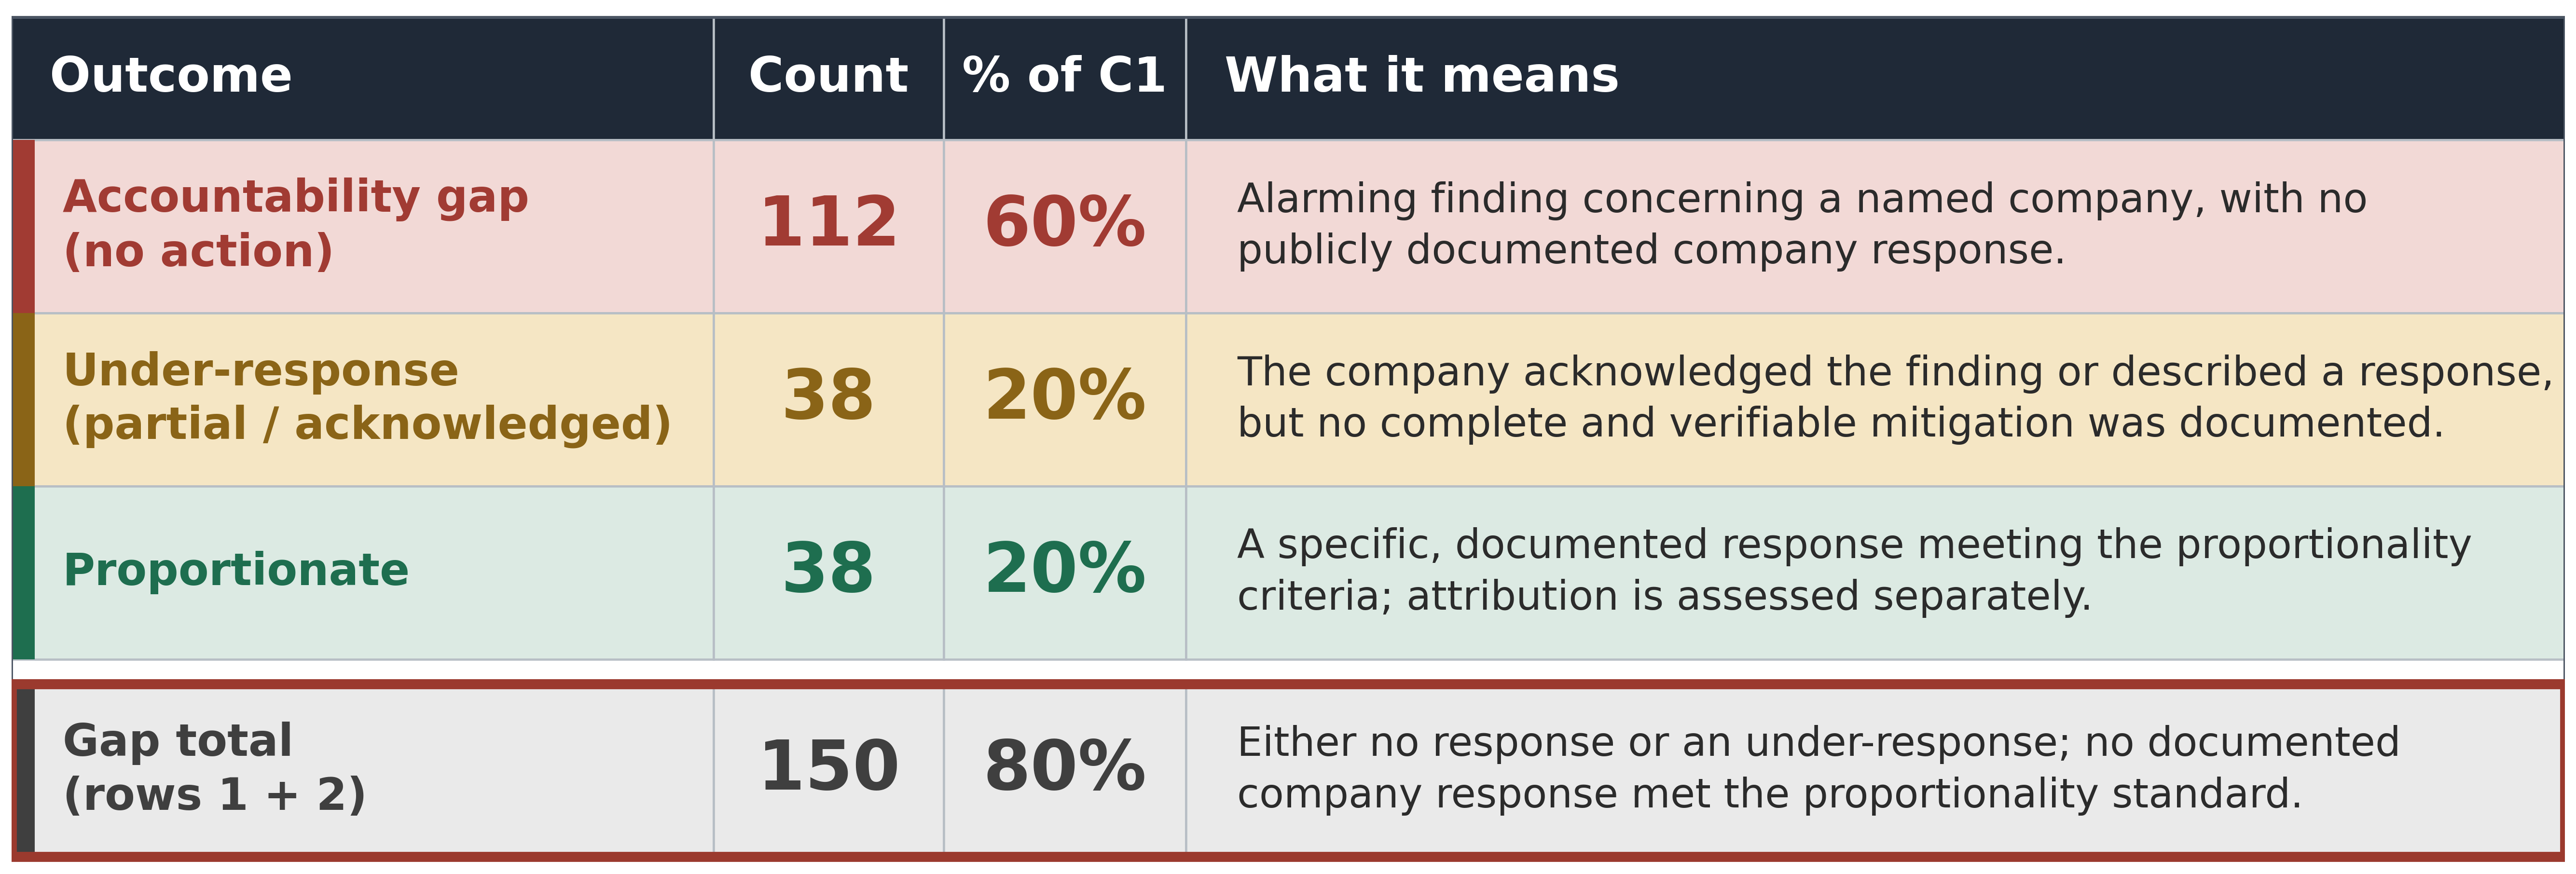
\includegraphics[width=\textwidth]{figures/figure1_headline_outcomes_table.png}
\end{minipage}
\par\medskip
\section{Background}\label{sec:background}
\subsection{Government AI institutes}
Government AI institutes emerged as technical public bodies focused on evaluating the safety of advanced AI systems. The first institutes were established in the United Kingdom, the United States, and Japan during 2023 and 2024. Their initial mandates broadly combined safety evaluation, research, standards development, and international cooperation~\citep{araujo2024}.

These institutes have since developed in different directions. In February 2025, the UK AI Safety Institute was renamed the AI Security Institute and its remit was refocused on risks with security implications, including cyberattacks, chemical and biological threats, fraud, and other forms of criminal misuse~\citep{ukaisi2025}. It remains within the Department for Science, Innovation and Technology and focuses on research and evaluation rather than regulatory enforcement. In June 2025, the US AI Safety Institute was re-established as the Center for AI Standards and Innovation (US CAISI) within the National Institute of Standards and Technology. Its work combines model evaluation and national-security assessment with measurement science, guidelines, and voluntary standards development~\citep{uscaisi2026}. Japan's AI Safety Institute, based within the Information-technology Promotion Agency, primarily develops evaluation methods, guidance, standards, and testing infrastructure~\citep{japanaisi2026}. France's INESIA, launched in 2025, is not a new standalone agency but a coordinated network of existing public bodies working on systemic-risk analysis, model evaluation, and support for the implementation of AI regulation~\citep{inesia2025}.

Government AI institutes therefore no longer represent a single institutional model. They vary in focus, structure, access arrangements, and connection to standards or regulatory processes. Most findings examined in this paper are technical outputs that may inform developers and policymakers but do not themselves compel a company response or remediation. We use ``government AI institutes'' as an umbrella term for the public bodies in our sampling frame that conduct or coordinate external evaluations of advanced AI systems. We distinguish them from independent evaluators while applying the same public-record response framework to findings reported by both groups.

\subsection{Independent AI system evaluators and third-party auditing}
 Independent evaluators are defined as non-government organisations (including non-profit organisations, for-profit evaluation firms, and academic research groups) that are institutionally separate from the developer whose system they evaluate and that conduct and publicly report frontier-AI evaluations. They include generalist evaluators such as METR and Apollo Research and domain-specific organisations such as SecureBio. Independent evaluators also test frontier systems for dangerous capabilities, safeguard failures, and other risks, but differ from government institutes in institutional status, funding, access arrangements, and public responsibilities. Their access may depend on voluntary developer cooperation, contractual arrangements, application programming interfaces, or publicly available models, allowing some to conduct pre-deployment evaluations while limiting others to post-deployment testing. At the same time, independent evaluators can provide specialised expertise and scrutiny outside both government and frontier-model developers. Recent work therefore treats evaluator independence, system access, methodological rigour, reporting arrangements, and audit standards as important dimensions of third-party auditing \citep{falco2021,costanzachock2023,brundage2026,birhane2024}. This paper treats government institutes and independent evaluators as distinct institutional categories while applying the same public-record response framework to eligible findings from both.

\section{Methodology}\label{sec:methods}
\subsection{Data collection}\label{sec:data}
We constructed the sampling frame by identifying 46 government bodies and independent evaluators that conducted frontier-AI evaluations and publicly reported their methods and results. We screened 6,684 publications and identified 457 reports containing sufficiently documented evaluations of advanced AI systems. The earliest included report was published on March 17, 2023, and the public-record cutoff was August 29, 2026. From these reports, we coded 1,146 distinct findings. The corpus includes adverse findings about named systems, findings about anonymised systems, reassuring or null results, capability trends, and methodology or governance findings. Section~\ref{sec:accountability} places them in three tiers. Only the 233 Tier A (trackable evaluation) findings---adverse findings about a named model or developer---enter the response and proportionality analyses. The sampling frame and the 46 reporting-institution labels, including separate labels for joint evaluations, are listed in Appendices~\ref{app:sampling} and~\ref{app:composition}.

The unit of analysis is an individual finding rather than a report. A finding is one discrete, evidence-backed, independently codeable claim concerning one accountable company. It must be asserted by the evaluator and supported by a measured result, observed behaviour, or documented process fact. Opinions, recommendations, announcements, and plans are excluded. Results are combined when they concern the same company, describe the same issue, and would reasonably call for a common response. They are coded separately when they describe substantively different issues or would reasonably call for different responses. Results concerning different companies are always coded as separate findings, even when the same report identifies the same problem in multiple companies' models. Results concerning multiple models from one company may be combined when they document the same issue and would reasonably call for the same response. Each finding receives a unique Finding ID, while findings drawn from the same report retain a common Report ID.

The corpus is restricted to evidence available in the public record. Findings communicated privately but not subsequently disclosed cannot be observed. We also excluded non-English-language outputs where a sufficiently reliable English version was unavailable. The resulting corpus should therefore be interpreted as a structured collection of publicly accessible, predominantly English-language evidence, not as a complete census of every evaluation performed by the included institutions.

\subsubsection{Tooling and human oversight}\label{sec:tooling-overview}
Corpus construction was AI-assisted. Automated screening and extraction identified candidate publications and findings, while AI agents searched separately for Channel A (company responses), Channel B (policy uptake), and Channel C (public coverage). Two authors independently reviewed each retained finding and its coding, including eligibility, tier, severity, response evidence, and Action Level; the agreed human judgment determined the final coding. Appendix~\ref{app:tooling} gives the search instructions, source classes, documented effort, and limitations.

\subsection{Defining the accountability set}\label{sec:accountability}
We assigned each finding to one of three mutually exclusive tiers based on whether it reported an adverse or safety-relevant result and permitted developer-specific response analysis.

Tier A (Trackable evaluation findings): Response-trackable adverse findings. A finding entered Tier A (Trackable evaluation findings) when it: (1) reported a specific adverse or safety-relevant result; (2) identified a named model, system, or developer rather than only an anonymised placeholder; and (3) concerned an issue within the developer's capacity to address, such that a company response could reasonably be assessed. These 233 findings constitute the accountability set and are the only findings included in the Action Level and proportionality analyses.

Tier B (Non-trackable evaluation findings): Empirical findings that did not meet at least one Tier A condition. These include anonymised-system results, reassuring or null results, bare scores or rankings without a concerning threshold, non-frontier systems, capability trends, inconclusive results, and findings for which a company response could not reasonably be assessed.

Tier C (Non-empirical findings): Methodology, framework, governance or process, tooling, milestone, and other findings that did not report empirical model behaviour or capability.

All three tiers remain in the descriptive corpus. Only Tier A (Trackable evaluation findings) enters the company-response and proportionality analyses.

\subsection{Severity of risk classification}\label{sec:severity}
A finding was classified as C1 (significant risk) when the reported evidence met at least one significant-risk threshold across eight risk domains: chemical, biological, radiological, and nuclear (CBRN) uplift; offensive cyber capability; autonomy, self-replication, or AI research-and-development (AI-R\&D) automation; persuasion or societal harm at scale; deliberate deception or misalignment; deployed-safeguard failure; compromised evaluation integrity; or acute individual harm. Findings could be assigned to more than one domain. A finding was classified as C2 (low risk) when the reported evidence did not meet any of these significant-risk thresholds. This does not necessarily mean that the finding was unimportant or that no response was warranted. The eight domains draw on two sources: published developer frameworks and additional risk criteria developed for this study. Domains D1--D3---CBRN uplift, offensive cyber capability, and autonomy including AI-R\&D automation and self-replication---correspond to dangerous-capability thresholds that frontier developers publish for their own systems in the Anthropic Responsible Scaling Policy~\citep{anthropic2026rsp}, the OpenAI Preparedness Framework~\citep{openai2025preparedness}, and the Google DeepMind Frontier Safety Framework~\citep{deepmind2026fsf}. Domains D4 and D5---persuasion or societal harm at scale and demonstrated deceptive misalignment---correspond to categories that those frameworks treat less uniformly. Domains D6--D8---deployed-safeguard failure, compromised evaluation integrity, and acute individual harm---are additional criteria developed for this study. They describe failures observed in the evaluation literature that the developers' capability thresholds do not cover.

The majority vote of the three models (Claude Sonnet 5, GPT-5.5, and Gemini 3.1 Pro) provided the initial severity classification. Two authors then independently reviewed every finding and its supporting evidence, including the individual model votes and rationales. Where warranted, the authors overrode the model majority; the agreed human-reviewed label was the final severity classification used in the analysis. Individual model votes and model-generated reasons were retained so that model disagreements remained observable. Appendix~\ref{app:severity} describes the annotation procedure; the complete prompt, boundary rules, and output format are available with the supplemental study materials.

Across the full corpus, 1,032 of 1,146 findings (90.1\%) received a unanimous 3--0 classification, while 114 (9.9\%) were determined by a 2--1 vote. Among the 233 Tier A (trackable evaluation) findings, 194 (83.3\%) received a unanimous classification and 39 (16.7\%) were determined by a 2--1 vote. The final corpus contained 340 C1 (significant risk) and 806 C2 (low risk) findings. Within Tier A (trackable evaluation), 190 findings were classified C1 (significant risk) and 43 were classified C2 (low risk).

\subsection{Response evidence and outcome coding}\label{sec:coding}
\subsubsection{Evidence channels}\label{sec:evidence-channels}
\noindent\begin{minipage}{\textwidth}
\centering
\refstepcounter{table}
\label{tab:evidence-channels}
\textbf{Table \thetable: Evidence channels searched separately through August 29, 2026. Channels B and C do not count as a company response.}\par\smallskip
\scriptsize
\setlength{\tabcolsep}{3pt}
\renewcommand{\arraystretch}{1.0}
\begin{tabularx}{\textwidth}{>{\raggedright\arraybackslash}p{0.18\linewidth} >{\raggedright\arraybackslash}p{0.53\linewidth} >{\raggedright\arraybackslash}X}
\toprule
Channel & Evidence examined & Role in the analysis \\
\midrule
Channel A (company response) & Company statements, system cards, and safety or deployment pages. & Attribution and Action Level. \\
Channel B (policy uptake) & Official parliamentary, legislative, regulatory, and government records. & Policy Level. \\
Channel C (public coverage) & Independent media coverage, academic citations, and notable public discussion. & External visibility. \\
\bottomrule
\end{tabularx}
\end{minipage}
\par\smallskip

The resulting public-record evidence was coded into four study-defined measures: Attribution, Action Level, Policy Level, and Proportionality.

\subsubsection{Attribution}\label{sec:attribution}
Attribution records whether an identified response was publicly connected to the relevant finding. (a) Explicit attribution: The responding company directly referenced the finding, report, evaluation result, or evaluating institution, or stated that its response was informed by that evidence. (b) No explicit attribution: A qualifying response was identified, but the company did not publicly state a connection to the finding. (c) No response located: No qualifying company response was identified, so attribution does not arise. Attribution is assessed only where a company response exists. Cases with no identified response are recorded under the third category rather than left blank, so that a searched-and-empty result is distinguishable from an uncoded one. Attribution measures the company's public explanation and does not independently establish causation.

\subsubsection{Action Level}\label{sec:action-level}
Action Level records the strength of the publicly documented company response identified through Channel A (Company response). (a) None: No public response could be identified through the search by the cutoff date. (b) Acknowledged: The company recognised the finding or underlying problem but specified no action. (c) Partial: The company documented an action that addressed only part of the identified problem or was expressly described as interim, limited, or incomplete. (d) Substantive: The company documented a specific mitigation, model change, safeguard, access restriction, or deployment decision that directly addressed the identified problem. Action Level measures the content of the public response. It does not establish whether the action was successfully implemented or effective in reducing the risk. Only public primary documentation issued by the responding company was admitted as Channel A evidence; evaluator statements, news coverage, and other third-party sources did not themselves qualify as company responses.

\subsubsection{Policy Level}\label{sec:policy-level}
Policy Level records whether the finding received documented uptake through Channel B (policy uptake) and whether it created an enforceable requirement. The categories are No policy uptake identified, Non-binding policy-related uptake, and Binding policy action.

\par
\noindent\begin{minipage}{\textwidth}
\centering
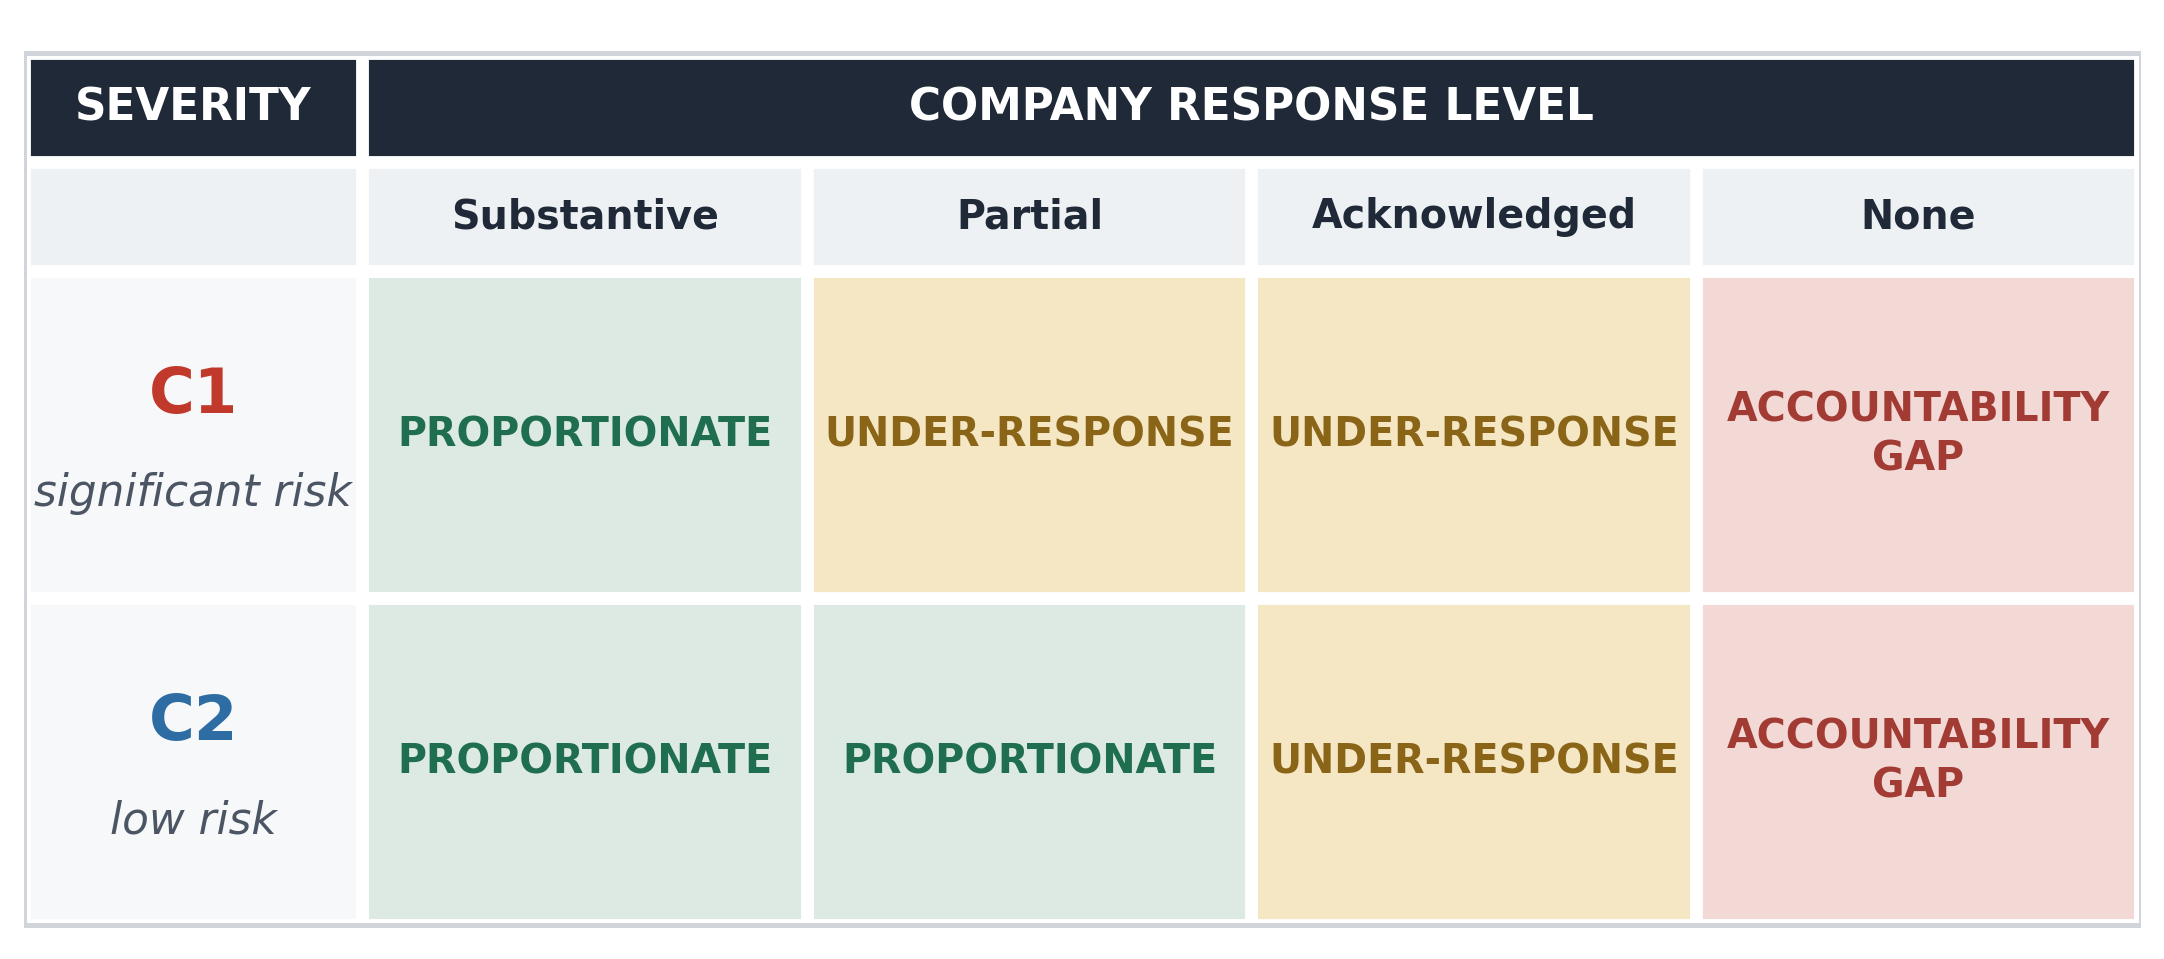
\includegraphics[width=0.92\textwidth]{figures/figure2_severity_matrix.png}
\par
\refstepcounter{figure}
\label{fig:severity-matrix}
\footnotesize\textbf{Figure \thefigure: Proportionality coding rule.} Rows show severity; columns show company-response level; cells show the resulting outcome. The matrix defines the rule, not observed results.
\end{minipage}
\par

\subsubsection{Proportionality}\label{sec:proportionality}
Proportionality combines two independently assigned classifications: finding severity and company Action Level. In Figure~\ref{fig:severity-matrix}, the rows show Severity (C1 significant risk or C2 low risk), and the columns show the documented company-response level. The matrix shows the severity-dependent rule used to classify every Tier A (trackable evaluation) finding. Equivalently, a C1 (significant risk) finding requires a Substantive response to meet the proportionality standard, whereas a C2 (low risk) finding requires at least a Partial response. Acknowledgment without action never meets the standard, and the absence of a company response always produces a no-action gap. This is a study-defined measure of documented response proportionality. It evaluates whether the publicly described response met the minimum Action Level associated with the finding's severity classification. It does not establish that the response was effective, that remediation was successfully implemented, or that the underlying risk was eliminated.

\section{Results}\label{sec:results}
We first report company-response outcomes among the 190 C1 (significant risk) findings in Tier A (trackable evaluation findings), which constitute the paper's primary accountability analysis. We then examine differences by evaluation-access type, public coverage of findings without company responses, and the extent to which reported company responses could be independently verified.

\subsection{Company responses to significant-risk findings}\label{sec:headline}
Restricted to C1 (significant risk) findings---the comparison relevant to the paper's central accountability question---152 of 190 findings (80\%; Wilson 95\% CI 74--85\%) received either no publicly documented company response or an inadequate one. This combined figure, rather than the 62.2\% no-response rate across all 233 Tier A (trackable evaluation) findings, is the paper's central result. Because it is calculated only over C1 findings, it is not mechanically affected by the number of C2 (low risk) findings included in the corpus. Of the 76 C1 findings with a located company response, 64 had explicit attribution and 12 did not. In Channel B (policy uptake), 41 C1 findings received non-binding policy uptake, one received binding action, and 148 had no identified policy uptake. Robustness checks and subgroup tests are reported in Appendix~\ref{app:robustness}.

\subsection{Outcomes by evaluation access type}\label{sec:access}
Among the C1 (significant risk) Tier A (trackable evaluation) findings classified as either pre- or post-deployment, the substantive-response rate was 55\% for the 44 pre-deployment findings and 7\% for the 131 post-deployment findings. Pre-deployment findings were therefore roughly eight times as likely to receive a substantive response. No-response rates also differed substantially: 6.8\% for pre-deployment findings and 79.4\% for post-deployment findings. A two-proportion test gave \emph{z} = -8.54, \emph{p} \textless{} 0.001, and the difference remained significant after adjustment for clustering within reports (\emph{p} \textless{} 0.001; Appendix~\ref{app:subgroups} and Figure~\ref{fig:appendix-gap-access}). These comparisons describe an association and should not be interpreted causally.

This descriptive association is consistent with pre-deployment access facilitating company action, although access type is correlated with evaluator, disclosure arrangements, domain, and other institutional differences. One plausible mechanism is visible in the case-level record: pre-deployment findings are communicated while the deployment decision window remains open and are frequently published under coordinated-disclosure arrangements. Forty-nine of the 88 recorded response lags were zero days, meaning that the finding and company response were published together. This remains a plausible interpretation rather than a mechanism established by the comparison itself.

\subsection{Public coverage of findings without company responses}\label{sec:traction}
Of the 114 C1 (significant risk) Tier A (trackable evaluation) findings classified as Accountability gap (no action), 91 (80\%) have at least one mainstream press item or academic citation recorded. Including notable public discussion, 92 (81\%) have evidence in at least one Channel C (public coverage) field. Thus, the absence of a publicly documented company response was not generally confined to findings with no observable external coverage. This evidence does not establish that the relevant company saw the coverage, but it shows that many no-response findings were publicly visible beyond the original evaluation report. The channel-by-channel breakdown and the inconclusive traction comparison are reported in Appendix~\ref{app:subgroups} and Table~\ref{tab:traction}.

\subsection{Independent verification of company responses}\label{sec:verification}
A company response does not necessarily permit independent verification. During its pre-deployment evaluation of GPT-5.5, UK AISI identified a universal jailbreak within six hours of testing \citep{openai2026gpt55}. OpenAI subsequently reported several changes to its safeguard stack. However, a configuration issue in the version supplied to UK AISI meant the institute could not verify the effectiveness of the final configuration before deployment; the cited source does not document a verified patch of the jailbreak.

This case illustrates the distinction captured by the Partial category: a company may document a response while the external evaluator remains unable to verify whether the final mitigation addressed the identified vulnerability.

The limitation this case exposes is structural rather than incidental. Channel A (company response) admits only the responding company's own primary documentation (Section~\ref{sec:coding}), so every one of the 76 C1 (significant risk) findings that drew a response is evidenced by that company's account of itself. That is a property of the coding rule, not a finding. The question the rule cannot answer is whether a second party ever confirmed that the described action was taken, or that it worked.

Reading the response record for each of those 76 findings, we identify one case in which an evaluator is documented as having re-tested a revised safeguard and endorsed it: the US Center for AI Standards and Innovation's (US CAISI's) examination of Anthropic's rebuilt cyber classifier, which occurred during the export-control process and before redeployment (Section~\ref{sec:fable}). We identify one case in which the evaluator states that it could not verify the claimed fix---the GPT-5.5 jailbreak described above. For the remaining 74, the public record contains the company's description and nothing independent against which to check it.

The count of independently verified remediations should be read as a lower bound. It reflects what the cited sources describe; a verification exercise that took place but was not reported would not appear. Four further candidates were examined and excluded: collaboration on pre-deployment capability testing is not confirmation of a remedy, a capability designation is not a verified mitigation, a developer confirming an attack is not a developer demonstrating a fix, and a company's assessment of its own model using its own tooling is not independent. The Partial category captures the subset where the shortfall is visible at coding time---21 of the 190 C1 findings (11\%)---but the broader position is that proportionality throughout this paper is assessed against what companies state they did, not against remediation anyone else has checked. Appendix~\ref{app:examples}, especially Tables~\ref{tab:worked-substantive} and~\ref{tab:worked-partial}, gives worked examples of this boundary.

\paragraph{Limitations.} These results describe the public record, not unreported company action, and do not establish that an evaluation caused a response. Findings also cluster within reports, so subgroup comparisons use report-level adjustments.

\section{Understanding the accountability gap}\label{sec:interpretation}
Section 4 documents the distribution of publicly observable responses but does not, by itself, explain why those outcomes occurred. This section examines two forms of follow-through: company remediation in two illustrative cases and policy-record responses to findings in the corpus. These analyses help identify circumstances associated with observable action, but they are neither causal estimates nor exhaustive explanations of the accountability gap. Section 6 separately compares the follow-up mechanisms available to government AI institutes with those used by established oversight institutions.

To illustrate how evaluation findings can be followed by documented remediation despite the broader accountability gap, we examine two cases with an unusually clear public sequence from technical evidence to developer response. Both are included in the corpus and coded as receiving a Substantive response. In the Fable 5 and Mythos 5 case, the triggering Amazon report falls outside the evaluator-scope sampling frame, but the later US CAISI safeguard-testing and redeployment record is included as finding USCAISI-2026-06-CYB2. The cases contrast legally consequential action through an existing government authority with voluntary remediation through iterative pre-deployment collaboration. They are illustrative rather than representative.

\subsection{Enforcement through an existing legal instrument: Fable 5 and Mythos 5}\label{sec:fable}
Anthropic launched Claude Fable 5 on June 9, 2026. According to Anthropic, the US government applied export controls to Fable 5 and Mythos 5 on June 12, requiring the company to prevent access by foreign nationals inside and outside the United States. But Anthropic suspended access to both models worldwide.

Anthropic reported that the directive followed government awareness of an Amazon research report describing a technique for bypassing Fable 5's safeguards. The technique caused the model to identify software vulnerabilities and, in one instance, produce code demonstrating how one vulnerability could be exploited. Anthropic subsequently trained an updated safety classifier and reported that it blocked the identified technique in more than 99\% of cases. Anthropic also reported that US CAISI tested both the previous and updated safeguards and considered them ``extraordinarily strong''; this does not establish that US CAISI independently produced the 99\% estimate. The controls were lifted on June 30. Fable 5 returned to global availability on July 1, while Mythos 5 was initially restored only to selected US organisations. \citep{anthropic2026fable}.

The triggering Amazon report is not a corpus finding because it does not satisfy the evaluator-scope criteria. The later US CAISI safeguard-testing and redeployment record is included as finding USCAISI-2026-06-CYB2, and is the one corpus response for which the public record states that an evaluator tested the revised safeguards. The public record therefore documents a comparatively complete accountability sequence: a technical problem was reported, a binding legal instrument imposed restrictions, the company implemented a mitigation, and a government evaluator examined the revised safeguards before the restrictions were lifted.

The case does not show that the US federal government possessed or exercised deployment authority. The legally consequential action came through the Department of Commerce's export-control powers, while US CAISI contributed technical testing within the resulting process. It therefore illustrates how evaluation expertise can support remediation when another institution supplies an existing legal pathway.

\subsection{Collaborative pre-deployment remediation: GPT-5.6}\label{sec:gpt56}
OpenAI's system card describes an iterative pre-deployment process rather than a single evaluation event. UK AISI received early access to GPT-5.6 Sol and extensive grey-box access to its safeguard system. Across several testing rounds, UK AISI reported universal cyber-domain jailbreaks, including attacks that enabled long-form agentic work involving vulnerability discovery and exploit development. OpenAI states that it improved the system in response to UK AISI's findings and, by launch, had reproduced and mitigated the specific jailbreaks UK AISI reported. The system card does not claim that the broader vulnerability class was eliminated: UK AISI expected further red-teaming to identify similar jailbreaks, and OpenAI committed to continued testing with the institute. \citep{openai2026gpt56}.

We code the response as Substantive because OpenAI publicly attributes implemented pre-deployment mitigation to the jailbreaks reported by UK AISI. This classification refers specifically to mitigation of the reported attacks; it does not imply that GPT-5.6 had become resistant to all similar jailbreaks. Unlike the Fable 5 case, no binding government order was involved. The documented response occurred through repeated testing, private disclosure, mitigation, and retesting within an existing evaluator--developer collaboration.

Together, the two cases illustrate distinct pathways from technical evidence to remediation. In the Fable 5 case, an existing legal instrument imposed consequences, while government evaluation supported verification of the revised safeguards. In the GPT-5.6 case, pre-deployment access and an established evaluator--developer collaboration were followed by documented voluntary mitigation. Neither case establishes that publication of an evaluation finding, by itself, reliably triggers follow-up.

\section{Institutional mechanisms for reducing the accountability gap}\label{sec:industries}
The accountability problem examined in this paper is not unique to AI governance. Established oversight systems distinguish between producing technically credible findings, obtaining a response, verifying corrective action, and possessing authority to compel or escalate action. We compare the UK AI Security Institute (UK AISI) and US Center for AI Standards and Innovation (US CAISI) with seven established oversight bodies in the United States and the United Kingdom, focusing on formal mechanisms for information access, designated recipients, response, remediation or escalation, verification, and continuing follow-up. These bodies differ substantially in mandate, subject matter, and enforcement authority and are not presented as direct institutional templates for frontier AI governance. The comparison instead identifies mechanisms through which technical findings can remain actionable and publicly visible after an investigation or evaluation has concluded.

Detailed histories of the National Transportation Safety Board (NTSB) and Public Company Accounting Oversight Board (PCAOB), together with the wider institutional comparison, are provided in Appendix~\ref{app:institutions} and Table~\ref{tab:institutional-comparison}~\citep{uscode1135,ntsb2024,gao2002,sec2003,pcaob2013}.

Neither precedent provides a ready-made model for frontier AI governance. The NTSB cannot force recipients to adopt its recommendations, while the PCAOB regulates auditors rather than directly compelling audited companies to remedy every adverse finding. Nor do these precedents establish that AI evaluation institutions have failed in the same ways. They instead separate two institutional questions that are often conflated: whether a system provides a formal pathway from technical findings to documented follow-up, and whether the evaluators themselves are subject to independent supervision. Applied to frontier AI evaluation, these precedents motivate asking who should respond to an adverse finding, who tracks and evaluates that response, who verifies claimed remediation, and who---if anyone---oversees the evaluators.

The comparative lesson is therefore institutional rather than sector-specific. Government frontier-AI evaluators need not themselves become comprehensive regulators for their findings to enter a more systematic accountability process. Technical evaluation could remain institutionally separate while findings are connected to designated recipients, response expectations or obligations, public status tracking, procedures for reviewing claimed remediation, and defined pathways for escalation or referral. These mechanisms would not guarantee that every finding is remediated or that every response reduces real-world risk, but they would make follow-through more consistent, attributable, verifiable, and publicly inspectable.

\section{Conclusion}\label{sec:conclusion}
Government AI institutes and independent evaluators increasingly provide evidence about frontier systems that would otherwise remain available only through developer self-reporting. The findings in this paper do not question the value of that technical work. They examine whether the public record shows that alarming findings concerning named systems were followed by responses proportionate to the identified risk.


Closing this public accountability gap does not necessarily require converting technical institutes into general-purpose AI regulators. Companies participating in government evaluations could publish finding-level responses stating whether they accept, dispute, plan to address, or have remediated a finding. Institutes could maintain a public response-status record, subject to legitimate security and confidentiality constraints, and distinguish claimed remediation from independently verified remediation. Evaluation agreements could also establish response timelines and specify what status information may be disclosed.

The public record currently provides limited grounds for confidence that government and independent frontier-AI evaluations consistently lead to substantive improvements in deployed-system safety. Creating a visible and repeatable pathway from finding to response, follow-up, and verification would make that confidence more warranted, and make the contribution of the evaluation ecosystem more publicly accessible.


\clearpage
\begingroup
\small
\begin{thebibliography}{99}

\bibitem[Shevlane et al.(2023)]{shevlane2023}
T. Shevlane, S. Farquhar, B. Garfinkel, et al. (2023).
Model evaluation for extreme risks.
\emph{arXiv preprint arXiv:2305.15324}.
\url{https://arxiv.org/abs/2305.15324}.

\bibitem[Araujo et al.(2024)]{araujo2024}
R. Araujo, K. Fort, and O. Guest (2024).
Understanding the first wave of AI Safety Institutes: Characteristics, functions, and challenges.
\emph{arXiv preprint arXiv:2410.09219}.
\url{https://arxiv.org/abs/2410.09219}.

\bibitem[UK Government(2025)]{ukaisi2025}
UK Government (2025).
\emph{Tackling AI security risks to unleash growth and deliver Plan for Change}.
\emph{Department for Science, Innovation and Technology}, February 14, 2025.
\url{https://www.gov.uk/government/news/tackling-ai-security-risks-to-unleash-growth-and-deliver-plan-for-change}.

\bibitem[US CAISI(2026)]{uscaisi2026}
Center for AI Standards and Innovation (2026).
\emph{Center for AI Standards and Innovation (CAISI)}.
National Institute of Standards and Technology.
\url{https://www.nist.gov/caisi}.

\bibitem[Japan AISI(2026)]{japanaisi2026}
Japan AI Safety Institute (2026).
\emph{Japan AI Safety Institute (J-AISI)}.
Information-technology Promotion Agency.
\url{https://aisi.go.jp/assets/pdf/20260708_AISI_en.pdf}.

\bibitem[French Government(2025)]{inesia2025}
French Government (2025).
Le Gouvernement annonce la cr\'eation de l'Institut national pour
l'\'evaluation et la s\'ecurit\'e de l'intelligence artificielle (INESIA).
\emph{Minist\`ere de l'\'Economie, des Finances et de la Souverainet\'e
industrielle et num\'erique}, January 31, 2025.
\href{https://presse.economie.gouv.fr/le-gouvernement-annonce-la-creation-de-linstitut-national-pour-levaluation-et-la-securite-de-lintelligence-artificielle-inesia/}{French Government announcement}.

\bibitem[Falco et al.(2021)]{falco2021}
G. Falco, B. Shneiderman, J. Badger, et al. (2021).
Governing AI safety through independent audits.
\emph{Nature Machine Intelligence}, 3, 566--571.
\url{https://doi.org/10.1038/s42256-021-00370-7}.

\bibitem[Costanza-Chock et al.(2023)]{costanzachock2023}
S. Costanza-Chock, E. Harvey, I. D. Raji, M. Czernuszenko, and J. Buolamwini (2023).
Who audits the auditors? Recommendations from a field scan of the algorithmic auditing ecosystem.
\emph{arXiv preprint arXiv:2310.02521}.
\url{https://arxiv.org/abs/2310.02521}.

\bibitem[Brundage et al.(2026)]{brundage2026}
M. Brundage, N. Dreksler, A. Homewood, et al. (2026).
Frontier AI auditing: Toward rigorous third-party assessment of safety and security practices at leading AI companies.
\emph{arXiv preprint arXiv:2601.11699}.
\url{https://arxiv.org/abs/2601.11699}.

\bibitem[Birhane et al.(2024)]{birhane2024}
A. Birhane, R. Steed, V. Ojewale, B. Vecchione, and I. D. Raji (2024).
AI auditing: The broken bus on the road to AI accountability.
\emph{arXiv preprint arXiv:2401.14462}.
\url{https://arxiv.org/abs/2401.14462}.

\bibitem[Anthropic(2026)]{anthropic2026rsp}
Anthropic (2026).
\emph{Responsible Scaling Policy, Version 3.4}.
Effective July 8, 2026.
\url{https://www.anthropic.com/responsible-scaling-policy}.

\bibitem[OpenAI(2025)]{openai2025preparedness}
OpenAI (2025).
\emph{Preparedness Framework, Version 2}.
Last updated April 15, 2025.
\url{https://cdn.openai.com/pdf/18a02b5d-6b67-4cec-ab64-68cdfbddebcd/preparedness-framework-v2.pdf}.

\bibitem[Google DeepMind(2026)]{deepmind2026fsf}
Google DeepMind (2026).
\emph{Frontier Safety Framework, Version 3.1}.
Published April 17, 2026.
\url{https://deepmind.google/frontier-safety/}.

\bibitem[OpenAI(2026)]{openai2026gpt55}
OpenAI (2026).
\emph{GPT-5.5 System Card: External Evaluations for Cyber Capabilities---UK AISI}.
\url{https://deploymentsafety.openai.com/gpt-5-5/external-evaluations-for-cyber-capabilities---uk-aisi}.

\bibitem[Anthropic(2026)]{anthropic2026fable}
Anthropic (2026).
\emph{Redeploying Fable 5}.
\url{https://www.anthropic.com/news/redeploying-fable-5}.

\bibitem[OpenAI(2026)]{openai2026gpt56}
OpenAI (2026).
\emph{GPT-5.6 System Card}.
\url{https://deploymentsafety.openai.com/gpt-5-6}.

\bibitem[U.S. Congress(2026)]{uscode1135}
U.S. Congress (2026).
\emph{49 U.S.C. Section 1135: Secretary of Transportation's Responses to Safety Recommendations}.
\url{https://uscode.house.gov/view.xhtml?req=%28title%3A49+section%3A1135+edition%3Aprelim%29}.

\bibitem[National Transportation Safety Board(2024)]{ntsb2024}
National Transportation Safety Board (2024).
\emph{Responding to Our Safety Recommendations}.
\url{https://www.ntsb.gov/investigations/Pages/RecipientTipRecommendations.aspx}.

\bibitem[U.S. General Accounting Office(2002)]{gao2002}
U.S. General Accounting Office (2002).
\emph{Protecting the Public Interest: Selected Governance, Regulatory Oversight, Auditing, Accounting, and Financial Reporting Issues}.
Report GAO-02-483T.
\url{https://www.gao.gov/products/gao-02-483t}.

\bibitem[U.S. Securities and Exchange Commission(2003)]{sec2003}
U.S. Securities and Exchange Commission (2003).
\emph{Order Regarding Section 101(d) of the Sarbanes--Oxley Act of 2002}.
Release Nos. 33-8223 and 34-47746.
\url{https://www.sec.gov/rules-regulations/2003/04/order-regarding-section-101d-sarbanes-oxley-act-2002}.

\bibitem[Public Company Accounting Oversight Board(2013)]{pcaob2013}
Public Company Accounting Oversight Board (2013).
\emph{Staff Guidance Concerning the Remediation Process}.
\url{https://pcaobus.org/oversight/inspections/remediation/remediation_process}.

\bibitem[U.S. Food and Drug Administration(n.d.)]{fda_warning}
U.S. Food and Drug Administration (n.d.).
\emph{About Warning and Close-Out Letters}.
Accessed September 7, 2026.
\url{https://www.fda.gov/inspections-compliance-enforcement-and-criminal-investigations/warning-letters/about-warning-and-close-out-letters}.

\bibitem[U.S. Nuclear Regulatory Commission(n.d.)]{nrc_inspection}
U.S. Nuclear Regulatory Commission (n.d.).
\emph{Inspection}.
Accessed September 7, 2026.
\url{https://www.nrc.gov/about-nrc/regulatory/safety-oversight}.

\bibitem[Office for Nuclear Regulation(n.d.)]{onr_regulation}
Office for Nuclear Regulation (n.d.).
\emph{How we regulate}.
Accessed September 7, 2026.
\url{https://www.onr.org.uk/our-work/how-we-regulate}.

\bibitem[Financial Conduct Authority(2026)]{fca_supervision}
Financial Conduct Authority (2026).
\emph{Our approach to supervision}.
Updated March 26, 2026.
\url{https://www.fca.org.uk/publications/corporate-documents/our-approach-to-supervision}.

\bibitem[UK Civil Aviation Authority(2023)]{caa_oversight}
UK Civil Aviation Authority (2023).
\emph{145.B.300 Oversight principles}.
\url{https://regulatorylibrary.caa.co.uk/1321-2014/Content/Document%20Structure/02%20145/2%20Regs/145.B.300%20Oversight%20principles.htm}.

\bibitem[UK Civil Aviation Authority(n.d.)]{caa_enforcement}
UK Civil Aviation Authority (n.d.).
\emph{Enforcement and prosecutions}.
Accessed September 7, 2026.
\url{https://www.caa.co.uk/about-us/the-civil-aviation-authority/enforcement/enforcement-and-prosecutions/}.

\bibitem[Raji et al.(2020)]{raji2020}
I. D. Raji, A. Smart, R. N. White, et al. (2020).
Closing the AI accountability gap: Defining an end-to-end framework for internal algorithmic auditing.
In \emph{Proceedings of the 2020 Conference on Fairness, Accountability, and Transparency}, pages 33--44.
\url{https://doi.org/10.1145/3351095.3372873}.

\bibitem[Mökander et al.(2024)]{mokander2023}
J. Mökander, J. Schuett, H. R. Kirk, and L. Floridi (2024).
Auditing large language models: A three-layered approach.
\emph{AI and Ethics}, 4, 1085--1115. First published online in 2023.
\url{https://doi.org/10.1007/s43681-023-00289-2}.

\bibitem[Anderljung et al.(2023)]{anderljung2023}
M. Anderljung, E. T. Smith, J. O'Brien, et al. (2023).
Towards publicly accountable frontier LLMs: Building an external scrutiny ecosystem under the ASPIRE framework.
\emph{arXiv preprint arXiv:2311.14711}.
\url{https://arxiv.org/abs/2311.14711}.

\bibitem[Raji et al.(2022)]{raji2022}
I. D. Raji, P. Xu, C. Honigsberg, and D. E. Ho (2022).
Outsider oversight: Designing a third party audit ecosystem for AI governance.
\emph{arXiv preprint arXiv:2206.04737}.
\url{https://arxiv.org/abs/2206.04737}.

\bibitem[Staufer et al.(2025)]{staufer2025}
L. Staufer, M. Yang, A. Reuel, and S. Casper (2025).
Audit cards: Contextualizing AI evaluations.
\emph{arXiv preprint arXiv:2504.13839}.
\url{https://arxiv.org/abs/2504.13839}.

\bibitem[Bengio et al.(2026)]{bengio2026}
Y. Bengio et al. (2026).
\emph{International AI Safety Report 2026}.
\url{https://arxiv.org/abs/2602.21012}.

\bibitem[Raji and Buolamwini(2019)]{raji2019}
I. D. Raji and J. Buolamwini (2019).
Actionable auditing: Investigating the impact of publicly naming biased performance results of commercial AI products.
In \emph{Proceedings of the 2019 AAAI/ACM Conference on AI, Ethics, and Society}, pages 429--435.
\url{https://doi.org/10.1145/3306618.3314244}.

\bibitem[Wang et al.(2025)]{wang2025}
J. Wang, K. Huang, K. Klyman, and R. Bommasani (2025).
Do AI companies make good on voluntary commitments to the White House?
\emph{arXiv preprint arXiv:2508.08345}.
\url{https://arxiv.org/abs/2508.08345}.

\bibitem[Rost(2026)]{rost2026}
T. Rost (2026).
From disclosure to self-referential opacity: Six dimensions of strain in current AI governance.
\emph{arXiv preprint arXiv:2604.14070}.
\url{https://arxiv.org/abs/2604.14070}.

\end{thebibliography}

\endgroup
\vspace{1em}
\appendix
\begin{center}
    {\LARGE\bfseries Appendix}
\end{center}
\vspace{0.5em}

\counterwithin{table}{section}
\counterwithin{figure}{section}
\section{Sampling frame and source eligibility}\label{app:sampling}
The appendices follow the research process: sampling and search (Appendices A--B), coding (Appendix C), corpus and response evidence (Appendices D--E), robustness and worked examples (Appendices F--G), institutional context and prior work (Appendices H--I), and reproducibility (Appendix J).

\subsection{Detailed eligibility and source scope}
The 1,146 evaluation findings included outputs from the UK AI Security Institute, the US Center for AI Standards and Innovation, national and joint evaluation initiatives involving Australia, France, Japan, Singapore, and South Korea, and exercises conducted through the International Network for Advanced AI Measurement, Evaluation and Science. The sampling frame also included third-party evaluators such as METR, SecureBio, Apollo Research, Palisade Research, and other non-profit, academic, and commercial evaluation organisations.

The initial screening roster was derived from three sources: national institutes and initiatives identified through the International Network for Advanced AI Measurement, Evaluation and Science; members of the AI Evaluators Forum plus evaluator organisations already represented in the developing corpus; and frontier-developer release sites, searched only for material explicitly attributed to an external evaluator. Organisations later found to be co-author affiliations rather than publishing evaluators, together with national institutes that produced no qualifying report, remain in Table~\ref{tab:sampling-frame} and the screening ledger as zero-yield records.

Third-party outputs were eligible whether or not the work was conducted with a government institute, provided that the public material identified the evaluator and tested system and documented the methods and results sufficiently to extract a finding. Relevant sources included formal evaluation reports, research publications, institute progress reports containing evaluation results, joint-testing publications, and company model or system cards that explicitly reported or linked to an external evaluation. Company materials describing only internal evaluations were not treated as independent evaluation reports.

Table~\ref{tab:sampling-frame} lists the organisations whose publications were screened to build the corpus, with the number of publications screened and reports included.

\begingroup
\small
\setlength{\tabcolsep}{3pt}
\renewcommand{\arraystretch}{1.08}
\begin{longtable}{>{\raggedright\arraybackslash}p{0.293\linewidth} >{\raggedright\arraybackslash}p{0.293\linewidth} >{\raggedright\arraybackslash}p{0.293\linewidth}}
\caption{The 46 organisations in the sampling frame.}\label{tab:sampling-frame}\\
\toprule
Organisation screened & Publications screened & Reports included \\
\midrule
\endfirsthead
\multicolumn{3}{r}{\small Table \thetable\ (continued)} \\
\toprule
Organisation screened & Publications screened & Reports included \\
\midrule
\endhead
RAND Corporation & 759 & 6 \\
Kenya (Ministry of ICT and Digital Economy - network member) & 628 & 0 \\
Allen Institute for AI (Ai2) & 547 & 0 \\
Holistic AI & 431 & 9 \\
Google DeepMind & 377 & 0 \\
Scale AI & 324 & 81 \\
Anthropic & 302 & 28 \\
Cisco (Robust Intelligence / Foundation AI) & 287 & 13 \\
Thorn & 270 & 0 \\
UC Berkeley & 269 & 0 \\
OpenAI & 166 & 20 \\
UK AI Security Institute (UK AISI) & 160 & 67 \\
Center for AI Safety (CAIS) & 156 & 13 \\
EPFL & 155 & 0 \\
Redwood Research & 137 & 15 \\
Tsinghua University CoAI Group & 136 & 3 \\
FAR.AI & 117 & 19 \\
Korea AI Safety Institute (K-AISI) & 105 & 4 \\
Japan AI Safety Institute (J-AISI) & 100 & 3 \\
METR & 93 & 49 \\
UL Research Institutes - Digital Safety Research Institute (DSRI) & 91 & 2 \\
Citadel AI & 86 & 1 \\
SecureBio & 84 & 11 \\
Collective Intelligence Project (Weval) & 81 & 27 \\
Shanghai AI Laboratory (AI45 Lab) & 74 & 22 \\
Yale University & 69 & 0 \\
Gray Swan AI & 65 & 6 \\
Stanford University & 65 & 0 \\
Apollo Research & 57 & 13 \\
Dreadnode & 56 & 16 \\
France INESIA (via PEReN / ANSSI / Inria / LNE) & 55 & 4 \\
LatticeFlow AI & 52 & 5 \\
US Center for AI Standards and Innovation (CAISI, NIST) & 49 & 7 \\
Canadian AI Safety Institute (CAISI Canada) & 46 & 0 \\
Meta & 44 & 1 \\
Princeton Holistic Agent Leaderboard (HAL) & 35 & 9 \\
Palisade Research & 28 & 15 \\
Transluce & 27 & 14 \\
University of Oxford & 25 & 0 \\
IndiaAI Safety Institute & 21 & 0 \\
Singapore AI Safety Institute (SG AISI) & 18 & 4 \\
Australian AI Safety Institute & 12 & 0 \\
EU AI Office (European Commission) & 9 & 0 \\
AI Verification and Evaluation Research Institute (AVERI) & 7 & 1 \\
Meridian Labs & 7 & 0 \\
Gray Swan AI + UK AISI (joint) & 2 & 2 \\
\bottomrule
\end{longtable}
\endgroup
The sampling ledger contains 6,684 screened publication records and 490 organisation--report inclusion entries. After deduplicating joint or collaborative reports credited to more than one screened organisation and applying the final corpus exclusions, these entries correspond to the 457 reports analysed in the paper. Organisations with zero included reports remain in the table so that the sampling frame records unsuccessful as well as successful searches.
\section{AI-assisted search and human oversight}\label{app:tooling}
Corpus construction was AI-assisted. This appendix records the search instructions, evidence rules, documented effort, and limits of the process.

\subsection{Publication screening and finding extraction}
A total of 6,684 publications were enumerated across the 46 organisations in Appendix~\ref{app:sampling}. Automated title-and-abstract triage resolved 5,453 records against the inclusion rules in Section~\ref{sec:data}; LLM-based search agents examined 885 records for which the title was insufficient; and later targeted passes resolved 346 records. Every screened publication, including exclusions, is recorded in \texttt{sweep/master\_ledger.csv}. Candidate findings were extracted from source documents by the same tooling. Each retained finding has a source URL and supporting quotation.

\subsection{Response and uptake searches}\label{app:response-search}
For every Tier A (trackable evaluation) finding, the search sought three separate outcomes by the August 29, 2026 cutoff: a company response through Channel A, policy uptake through Channel B, and independent coverage through Channel C. These are claims about what the search located in public sources, not claims about everything that may exist.

\paragraph{Channel A (company response)}
Agents searched five source classes in order: (1) the accountable developer's newsroom, blog, or research index; (2) later model and system cards in the affected model family; (3) the developer's safety or deployment-safety pages; (4) official developer accounts and statements; and (5) open-web results used only to locate a company primary source. Queries combined the developer, evaluator, report, and specific finding. A standing policy that predated the finding did not qualify. Neither third-party reporting nor company work on the same general topic counted unless a company primary source addressed the finding. Each company-specific row received its own search, including rows split from one report.

\paragraph{Channel B (policy uptake)}
Agents searched official parliamentary, congressional, agency, legislative, and regulatory sources using the evaluator name, report title, and report identifier. General policy activity on the same topic did not qualify without an explicit connection to the finding, report, or evaluator. An incomplete search was recorded as missing rather than as no uptake.

\paragraph{Channel C (public coverage)}
Agents searched independent media, academic citations, and notable public discussion. Sources included Google News results checked against the original outlet, Semantic Scholar by paper identifier, Google Scholar, and archived pages where necessary. The evaluator's own publicity and the company's own promotion were excluded. When a source could not be searched reliably, the log records the access problem rather than a negative result.

\paragraph{Retrieval and review}
The shared retrieval script attempted a direct request, extracted PDF or HTML text, and used an archived copy after access errors. This prevented a blocked page from being recorded as an absence. An independent AI-agent pass re-examined proposed Action Level codings against the cited evidence. Two authors then reviewed each retained finding and its coding; the agreed human judgment determined the final record.

\subsection{Documented effort and limitations}
The response search was conducted interactively by AI agents following the common source classes and admissibility rules above; it was not driven by a frozen prompt. Exact query-level replication is therefore not possible. The dated row-level logs are the evidence of what was searched and found.

\begingroup
\small
\setlength{\tabcolsep}{4pt}
\renewcommand{\arraystretch}{1.08}
\begin{longtable}{>{\raggedright\arraybackslash}p{0.58\linewidth} >{\raggedright\arraybackslash}p{0.32\linewidth}}
\caption{Documented response-search effort for Tier A (trackable evaluation) findings.}\label{tab:search-effort}\\
\toprule
Measure & Recorded value \\
\midrule
\endfirsthead
\multicolumn{2}{r}{\small Table \thetable\ (continued)} \\
\toprule
Measure & Recorded value \\
\midrule
\endhead
Tier A findings & 233 \\
Rows with a dated Channel A search log & 217 \\
Distinct search dates & 129 \\
Logs that enumerate searched sources & 119 \\
Logs that record a re-attempt after an access failure & 58 \\
Channel A log length, mean / median / maximum & 867 / 700 / 2,300 characters \\
Rows with Channel B evidence recorded & 233 (100\%) \\
Rows with any Channel C field populated & 200 (85.8\%) \\
\bottomrule
\end{longtable}
\endgroup

All 114 C1 (significant risk) findings coded None have a dated Channel A search log. The 16 Tier A rows without such a log are positive-response rows supported by located response evidence; they are not used to support a no-response classification. Search depth is still uneven, and no blind re-search was performed to estimate recall. Model-call and token counts were not instrumented, so they are not reported. Severity classification used a separate frozen prompt and three-model ensemble, described in Appendix~\ref{app:severity}.

\section{Tier taxonomy and severity annotation}\label{app:severity}
Every finding was assigned to one of three mutually exclusive tiers. Tier A (trackable evaluation findings) contains concerning empirical findings about a named frontier model or developer for which a company response could reasonably be assessed. Tier B (non-trackable evaluation findings) contains empirical findings that fail at least one Tier A condition, including anonymised, reassuring, null, inconclusive, bare-score, non-frontier, or capability-trend results. Tier C (non-empirical findings) contains methodology, framework, governance or process, tooling, milestone, and other non-empirical findings. Only Tier A enters the response analysis.

\par\medskip
\noindent\begin{minipage}[t]{0.55\textwidth}
\vspace{0pt}
\centering
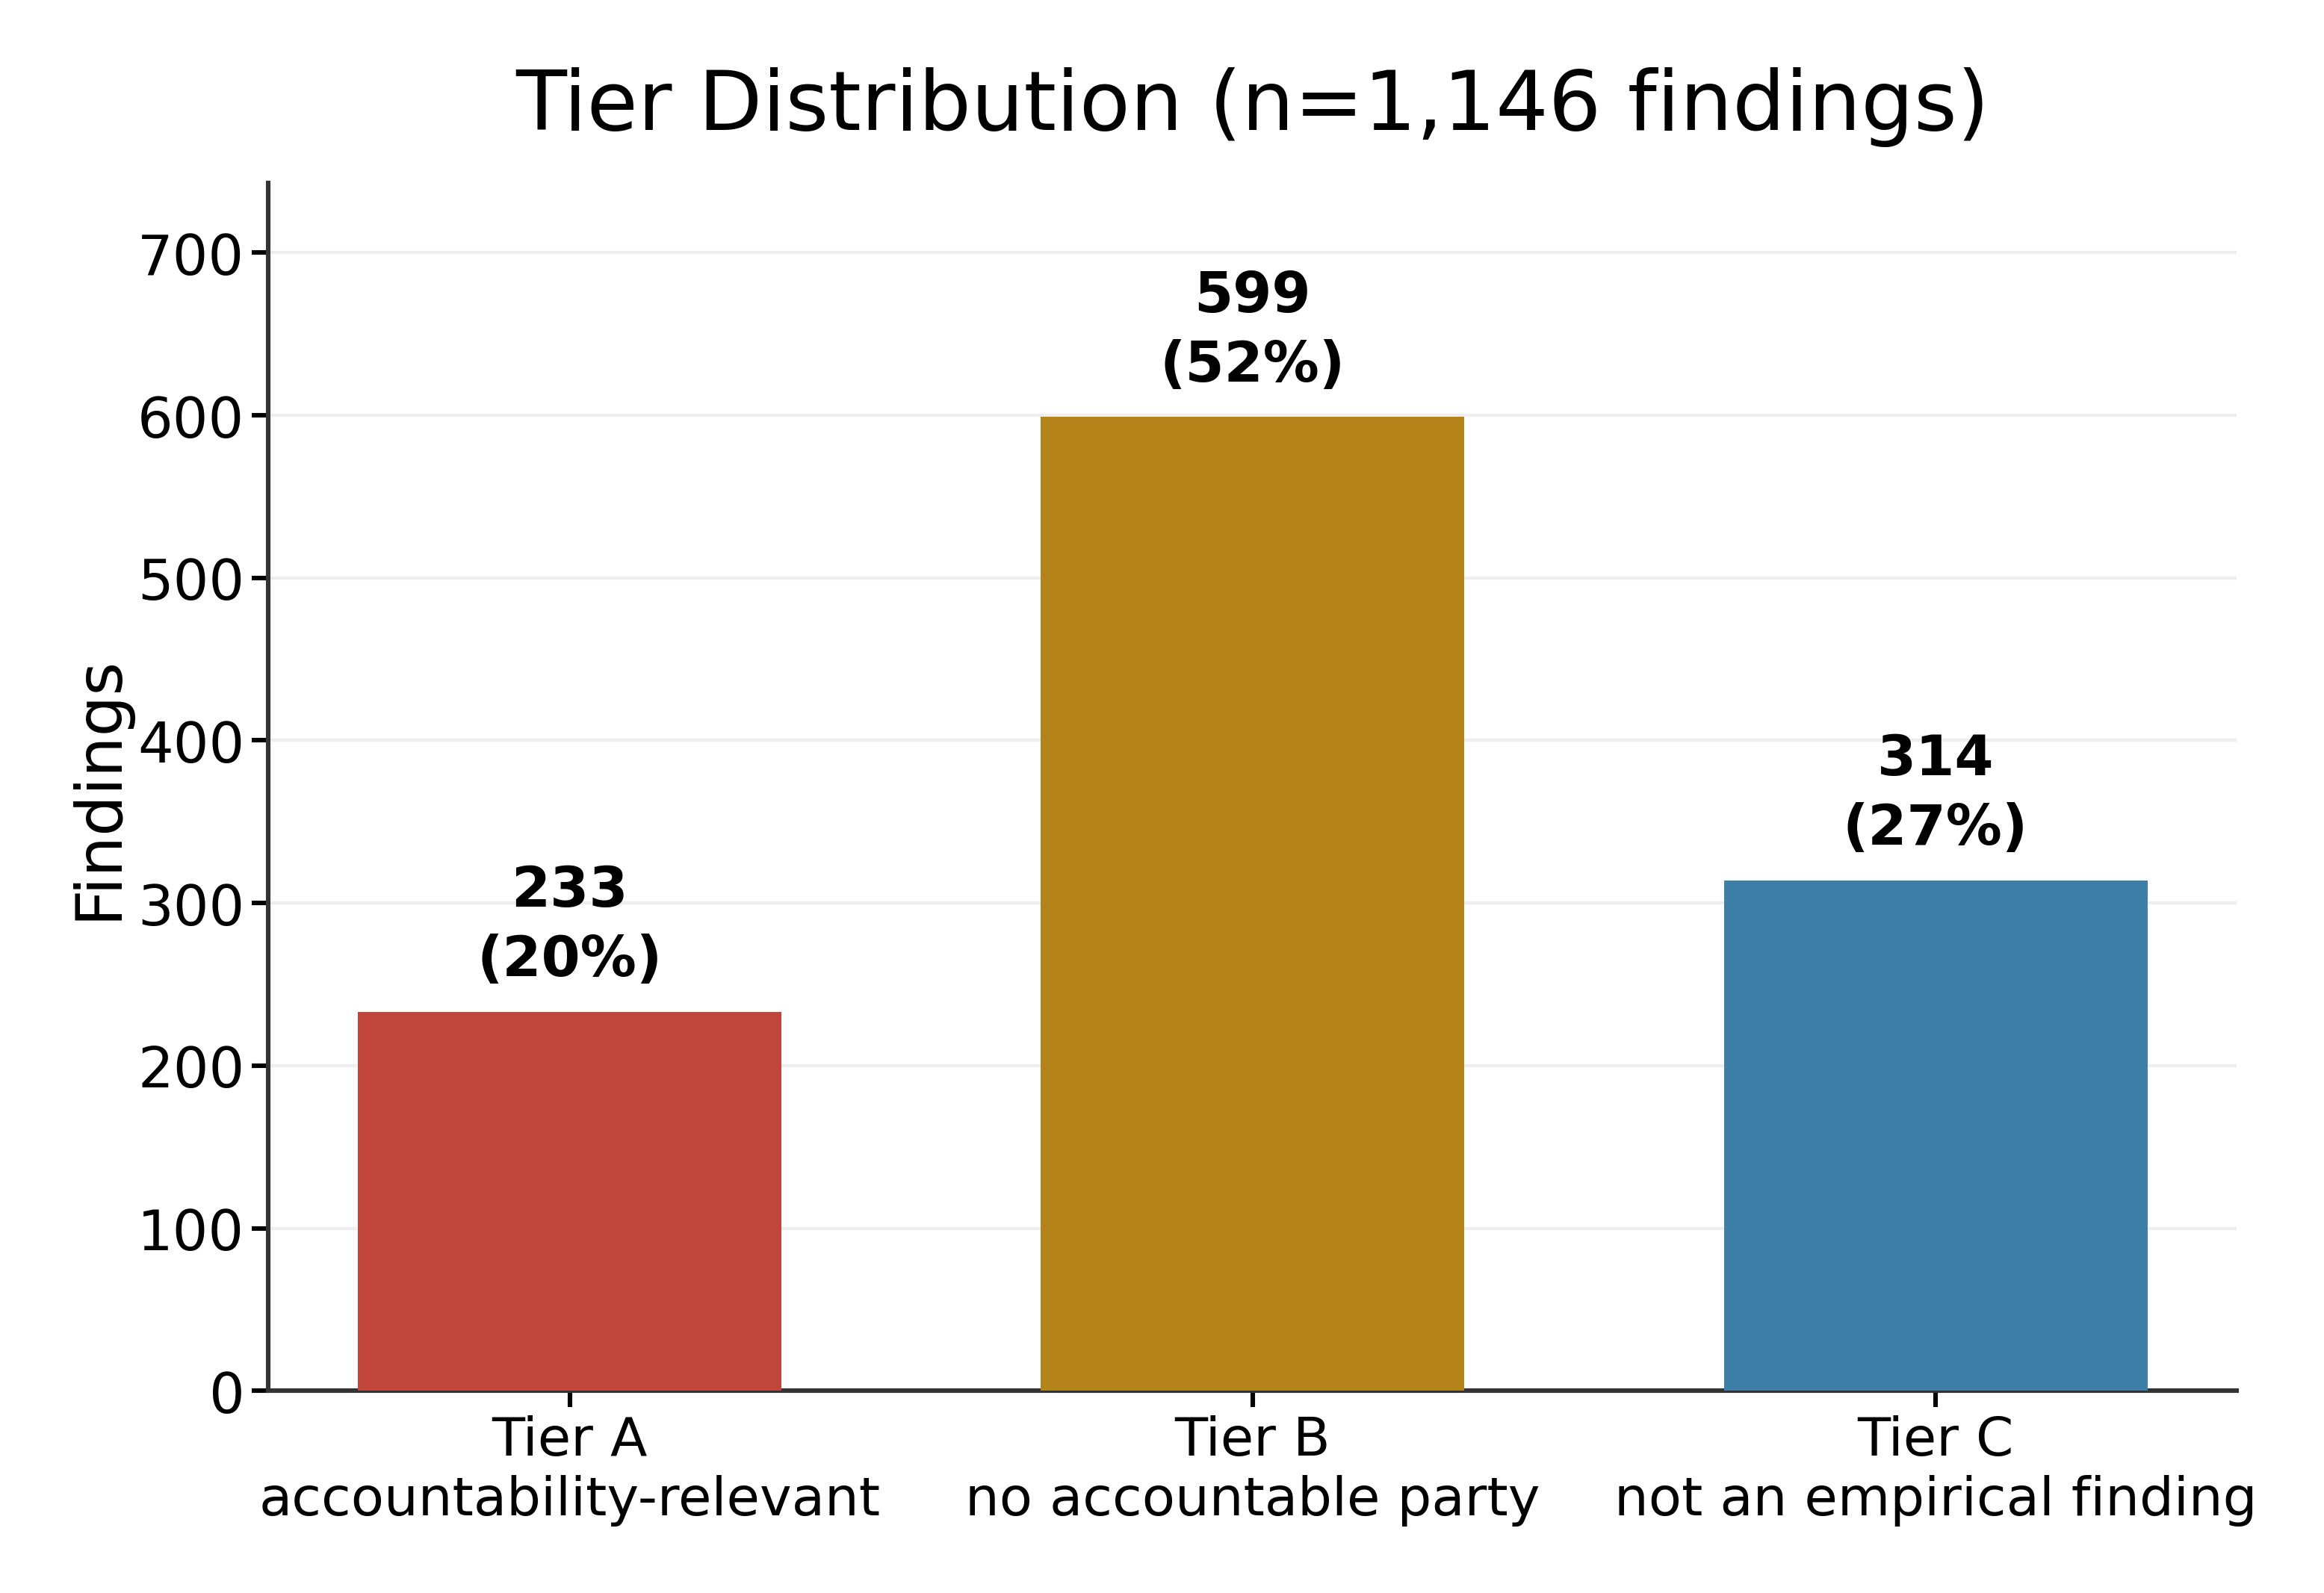
\includegraphics[width=0.96\linewidth,height=0.43\textheight,keepaspectratio]{figures/appendix_tier_distribution.png}
\par\smallskip
\refstepcounter{figure}
\label{fig:appendix-tier-distribution}
\small\textbf{Figure \thefigure:} The three-tier taxonomy across the 1,146-finding corpus: Tier A (trackable evaluation findings), 233 (20\%); Tier B (non-trackable evaluation findings), 599 (52\%); and Tier C (non-empirical findings), 314 (27\%). Only Tier A enters the response analysis.
\end{minipage}\hfill
\begin{minipage}[t]{0.41\textwidth}
\vspace{0pt}
\subsection{Severity domains and final review}
The severity prompt tests eight domains: chemical, biological, radiological, and nuclear (CBRN) and bio-chemical uplift; offensive cyber capability; autonomy, AI research-and-development (AI-R\&D) automation, and self-replication; persuasion or societal harm at scale; deliberate deception or misalignment; deployed-safeguard failure; compromised evaluation integrity; and acute individual harm. Each finding was independently classified by Claude Sonnet 5, GPT-5.5, and Gemini 3.1 Pro. Their majority vote produced the provisional C1 (significant risk) or C2 (low risk) label. Two authors then independently reviewed every finding and the model rationales and, where warranted, overrode the majority; the agreed human-reviewed label is the final severity classification used in the analysis.
\end{minipage}
\par\medskip

\begingroup
\small
\setlength{\tabcolsep}{3pt}
\renewcommand{\arraystretch}{1.08}
\begin{longtable}{>{\raggedright\arraybackslash}p{0.176\linewidth} >{\raggedright\arraybackslash}p{0.176\linewidth} >{\raggedright\arraybackslash}p{0.176\linewidth} >{\raggedright\arraybackslash}p{0.176\linewidth} >{\raggedright\arraybackslash}p{0.176\linewidth}}
\caption{Raw ensemble agreement. 1,032 of 1,146 findings received a unanimous 3--0 vote and 114 received a 2--1 vote. After human review, the final corpus contained 340 C1 (significant risk) and 806 C2 (low risk) findings.}\label{tab:ensemble}\\
\toprule
Subset & n & Unanimous & Split & Agreement rate \\
\midrule
\endfirsthead
\multicolumn{5}{r}{\small Table \thetable\ (continued)} \\
\toprule
Subset & n & Unanimous & Split & Agreement rate \\
\midrule
\endhead
All findings & 1,146 & 1,032 & 114 & 90.1\% \\
Tier A (Trackable evaluation findings) only & 233 & 194 & 39 & 83.3\% \\
\bottomrule
\end{longtable}
\endgroup
Model votes, retained rationales, and final labels are available with the study materials. \url{https://kunalssingh.com/evaluating-the-evaluators/\#data}

\subsection{Complete severity prompt (version 1.1)}
The following is the complete frozen prompt used for the reported severity classification. The system prompt was sent unchanged to all three ensemble models. The fields in braces in the user-message template were replaced with the corresponding finding-level values.

{\scriptsize
\verbatiminput{supplement/severity_prompt.txt}
}
\section{Corpus composition}\label{app:composition}
The corpus contains 46 distinct reporting-institution labels, including separate labels for joint evaluations and collaborations. Appendix~\ref{app:sampling} lists the separate 46-organisation screening frame; the equal totals are coincidental because the two lists do not contain exactly the same entities.
In the table, UK AISI denotes the institution now called the UK AI Security Institute (formerly the UK AI Safety Institute), and US CAISI denotes the US Center for AI Standards and Innovation; other national AISI labels denote the corresponding national AI Safety Institute.

\begingroup
\small
\setlength{\tabcolsep}{3pt}
\renewcommand{\arraystretch}{1.08}
\begin{longtable}{>{\raggedright\arraybackslash}p{0.38\linewidth} r >{\raggedright\arraybackslash}p{0.38\linewidth} r}
\caption{All 46 reporting-institution labels in the study dataset, ordered by findings down the left column and then the right. A label may denote a standalone institution, a collaboration, or a joint evaluation.}\label{tab:reporting-institutions}\\
\toprule
Reporting institution & Findings & Reporting institution & Findings \\
\midrule
\endfirsthead
\multicolumn{4}{r}{\small Table \thetable\ (continued)} \\
\toprule
Reporting institution & Findings & Reporting institution & Findings \\
\midrule
\endhead
UK AI Safety Institute (UK AISI) & 205 & Apollo Research + Anthropic (Apollo in the AI Safety Institute Consortium, AISIC) & 6 \\
Scale AI & 152 & LatticeFlow AI & 6 \\
METR & 113 & Princeton CRUX & 6 \\
Collective Intelligence Project (Weval) & 78 & AI Verification and Evaluation Research Institute (AVERI) & 5 \\
Shanghai AI Laboratory (AI45 Lab) & 74 & Joint UK + US + Singapore AISIs (International Network) & 4 \\
SecureBio & 48 & Joint UK AISI + OpenAI (company-published) & 4 \\
Apollo Research & 46 & Redwood Research + Scale AI & 4 \\
Transluce & 41 & Joint UK AISI + US CAISI + Gray Swan & 3 \\
FAR.AI & 39 & Singapore AI Safety Institute (SGAISI) / IMDA & 3 \\
Joint UK AISI + US CAISI & 37 & Japan AI Safety Institute (J-AISI) & 2 \\
US Center for AI Standards and Innovation (US CAISI) & 34 & Joint UK AISI + International Network (10 countries) & 2 \\
Center for AI Safety (CAIS) & 32 & Joint UK AISI + US CAISI + Anthropic & 2 \\
Dreadnode & 31 & Korea AI Safety Institute (K-AISI) & 2 \\
Redwood Research & 29 & RAND Europe & 2 \\
Princeton Holistic Agent Leaderboard (HAL) & 27 & Signature Science & 2 \\
Palisade Research & 19 & Singapore AI Safety Institute (SGAISI) / Korea AI Safety Institute (KR AISI) & 2 \\
RAND & 18 & UK AISI + Thorn & 2 \\
Holistic AI & 13 & Andon Labs & 1 \\
Gray Swan AI & 11 & Citadel AI & 1 \\
Cisco (Robust Intelligence / Foundation AI) & 10 & METR + Epoch AI & 1 \\
Irregular & 10 & Singapore AISI + Korea AISI (bilateral, network members) & 1 \\
France PEReN/INESIA & 9 & UK AISI + Anthropic + Theorem + MATS & 1 \\
International Network of AI Safety Institutes & 7 & UL Research Institutes (DSRI) & 1 \\
\bottomrule
\end{longtable}
\endgroup

Figure~\ref{fig:appendix-institution-tree} complements the complete list above by showing how reporting volume is distributed across institution types. It preserves the 1,146-finding total while showing the five largest reporting institutions in each group; the remaining institutions are combined as ``Other institutions.''

\par\medskip
\noindent\begin{minipage}{\textwidth}
\centering
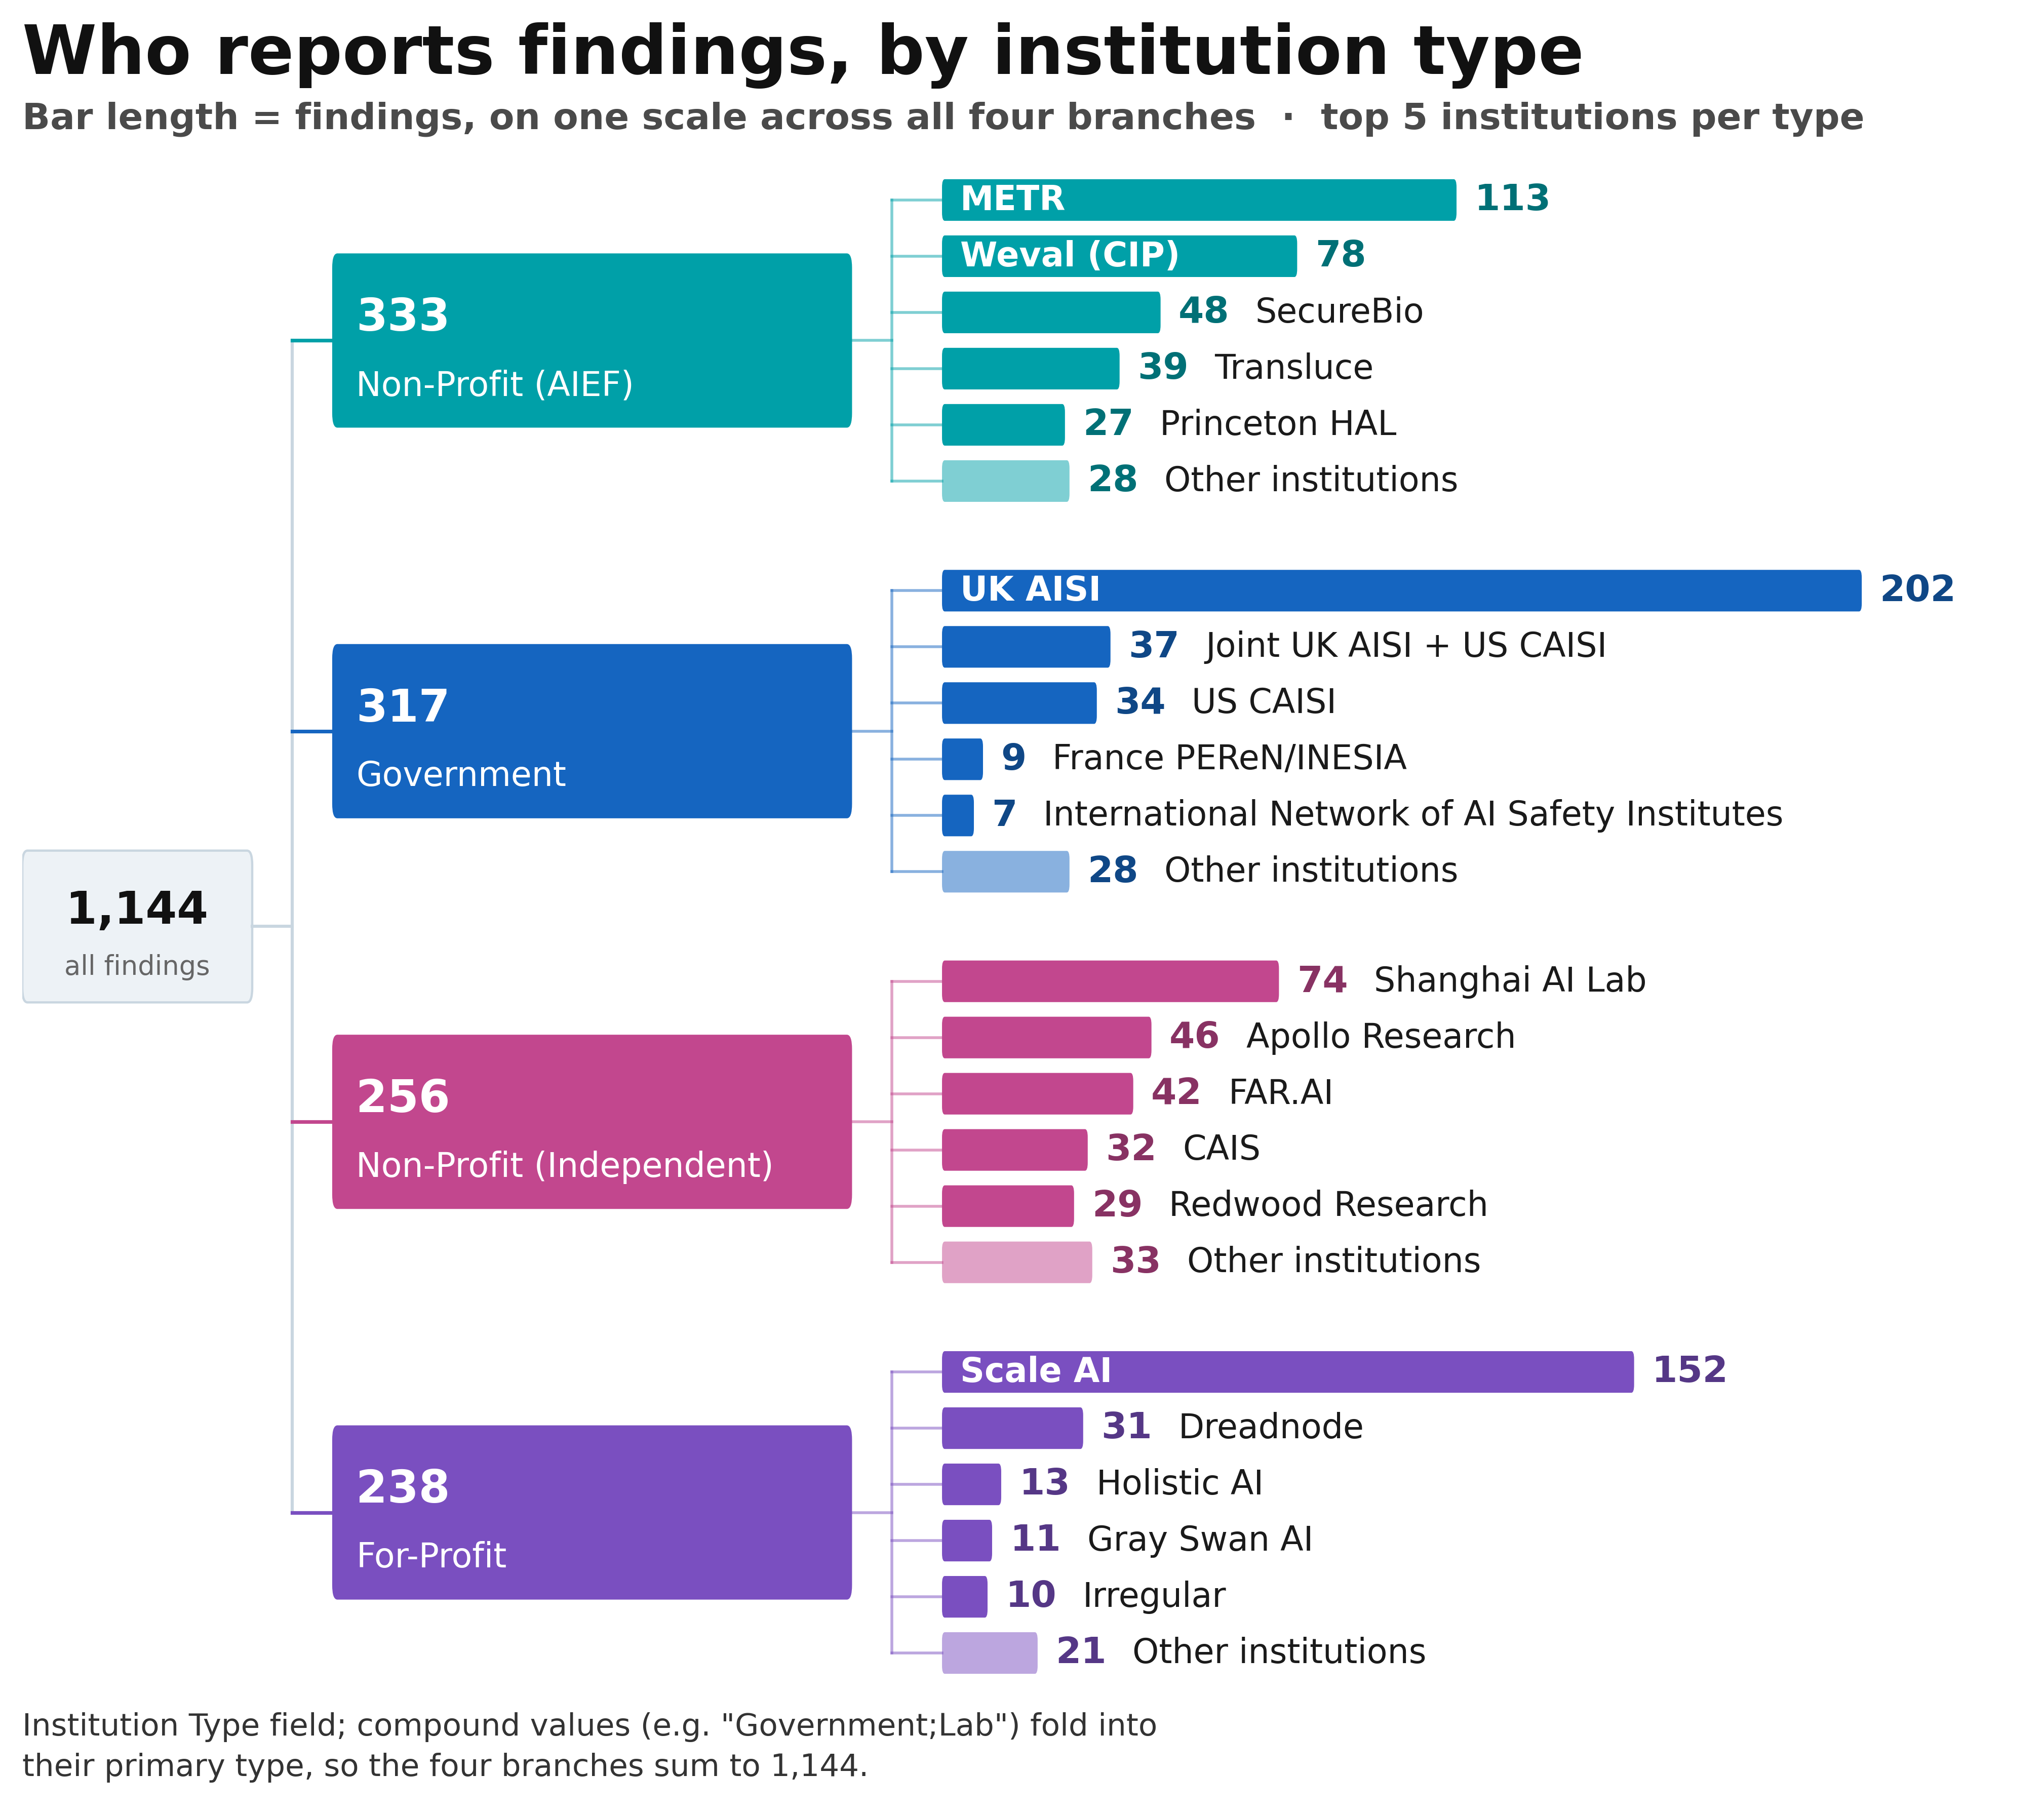
\includegraphics[width=0.98\linewidth,height=0.80\textheight,keepaspectratio]{figures/appendix_institution_tree.png}
\par\smallskip
\refstepcounter{figure}
\label{fig:appendix-institution-tree}
\small\textbf{Figure \thefigure:} Reporting volume by institution type across all 1,146 findings. Bar lengths use one common scale across the four groups. Institution types follow the dataset's Institution Type field. Compound values are assigned to their primary type, so the four groups sum to 1,146. The figure describes corpus composition, not evaluator quality or independence.
\end{minipage}
\par\medskip
\section{Response evidence and data access}\label{app:responses}
Complete finding-level rows and supporting evidence are available through the study website below. Among the 38 C1 (significant risk) Tier A (trackable evaluation) findings coded Substantive, 35 carry Explicit attribution---the company named the evaluator or finding in its response; the three exceptions drew a substantive fix with no explicit public credit to the evaluator.

\noindent\textbf{Complete rows and supporting data:} \url{https://kunalssingh.com/evaluating-the-evaluators/\#data}
\section{Robustness and subgroup analyses}\label{app:robustness}
Core corpus statistics were independently recomputed from the study dataset; the reproduction path is documented in Appendix~\ref{app:reproducibility}. Throughout this appendix, Tier A means trackable evaluation findings, C1 means significant risk, and C2 means low risk.

\begingroup
\raggedbottom
\subsection{Is the headline an artefact of the counting unit?}
The headline counts findings. Because one report can yield several findings, a small number of heavily split reports could in principle drive the result. It does not: the shortfall rate remains high under each alternative unit.

\begingroup
\small
\setlength{\tabcolsep}{3pt}
\renewcommand{\arraystretch}{1.08}
\begin{longtable}{>{\raggedright\arraybackslash}p{0.220\linewidth} >{\raggedright\arraybackslash}p{0.220\linewidth} >{\raggedright\arraybackslash}p{0.220\linewidth} >{\raggedright\arraybackslash}p{0.220\linewidth}}
\caption{Robustness of the headline shortfall to alternative counting units.}\label{tab:robustness}\\
\toprule
Unit of analysis & Shortfall & Rate & Wilson 95\% CI \\
\midrule
\endfirsthead
\multicolumn{4}{r}{\small Table \thetable\ (continued)} \\
\toprule
Unit of analysis & Shortfall & Rate & Wilson 95\% CI \\
\midrule
\endhead
Finding-weighted (headline) & 152/190 & 80.0\% & 74--85\% \\
Report-weighted (a report counts once) & 86/102 & 84.3\% & 76--90\% \\
Institution-weighted (mean of per-institution rates, n=25) & --- & 76.2\% & --- \\
All Tier A, ignoring severity & 188/233 & 80.7\% & 75--85\% \\
C2 (low risk) findings only & 36/43 & 83.7\% & 70--92\% \\
\bottomrule
\end{longtable}
\endgroup
Table~\ref{tab:robustness} shows that the result remains high under alternative counting units, ranging from 76.2\% under institution weighting to 84.3\% under report weighting.

\subsection{Uncertainty and subgroup comparisons}\label{app:subgroups}
The headline is a description of an enumerated public record rather than an estimate from a sample, so we do not attach a significance test to it. Table~\ref{tab:robustness} instead reports the result under five counting units, with Wilson intervals where applicable. Two subgroup comparisons support claims in the main paper and are reported here with their limits.

\noindent\textbf{Access type.}
Among C1 (significant risk) Tier A (trackable evaluation) findings, 3 of 44 pre-deployment findings received no response (6.8\%), compared with 104 of 131 post-deployment findings (79.4\%); the 15 Mixed findings are excluded. A two-proportion test gives \emph{z} = -8.54, \emph{p} \textless{} 0.001. The difference remains below \emph{p} \textless{} 0.001 after adjustment for clustering within reports.

\noindent\textbf{Severity.}
C1 (significant risk) findings received no response in 114 of 190 cases (60.0\%), compared with 31 of 43 C2 (low risk) findings (72.1\%); \emph{z} = -1.48, \emph{p} = 0.140. This is not evidence of no difference; the corpus cannot resolve whether severity predicts response.

\noindent\textbf{Clustering caveat.}
The 190 C1 Tier A findings sit in 102 reports, and outcomes cluster within reports because findings from the same report usually share an evaluator, disclosure arrangement, and developer. The estimated intra-cluster correlation is 0.626. The resulting design effect is 1.54, reducing the effective sample size from 190 to about 124; the design-effect-adjusted interval for the 80.0\% headline shortfall is 71.9--86.0\%. Two-proportion tests that treat findings as independent can therefore overstate significance; comparisons near the conventional threshold are reported descriptively rather than as demonstrated effects.

Two additional comparisons are descriptive. Government AISI findings fell short in 42 of 59 cases (71.2\%), compared with 110 of 131 (84.0\%) for third-party evaluators. The naive test gives \emph{p} = 0.042, but the difference does not remain below 0.05 after the report-clustering adjustment. Among C1 Tier A findings, 92 of 158 findings with documented public traction received no response (58.2\%), compared with 22 of 32 without documented traction (68.8\%); this comparison remains inconclusive.

\par\medskip
\noindent\begin{minipage}{\textwidth}
\centering
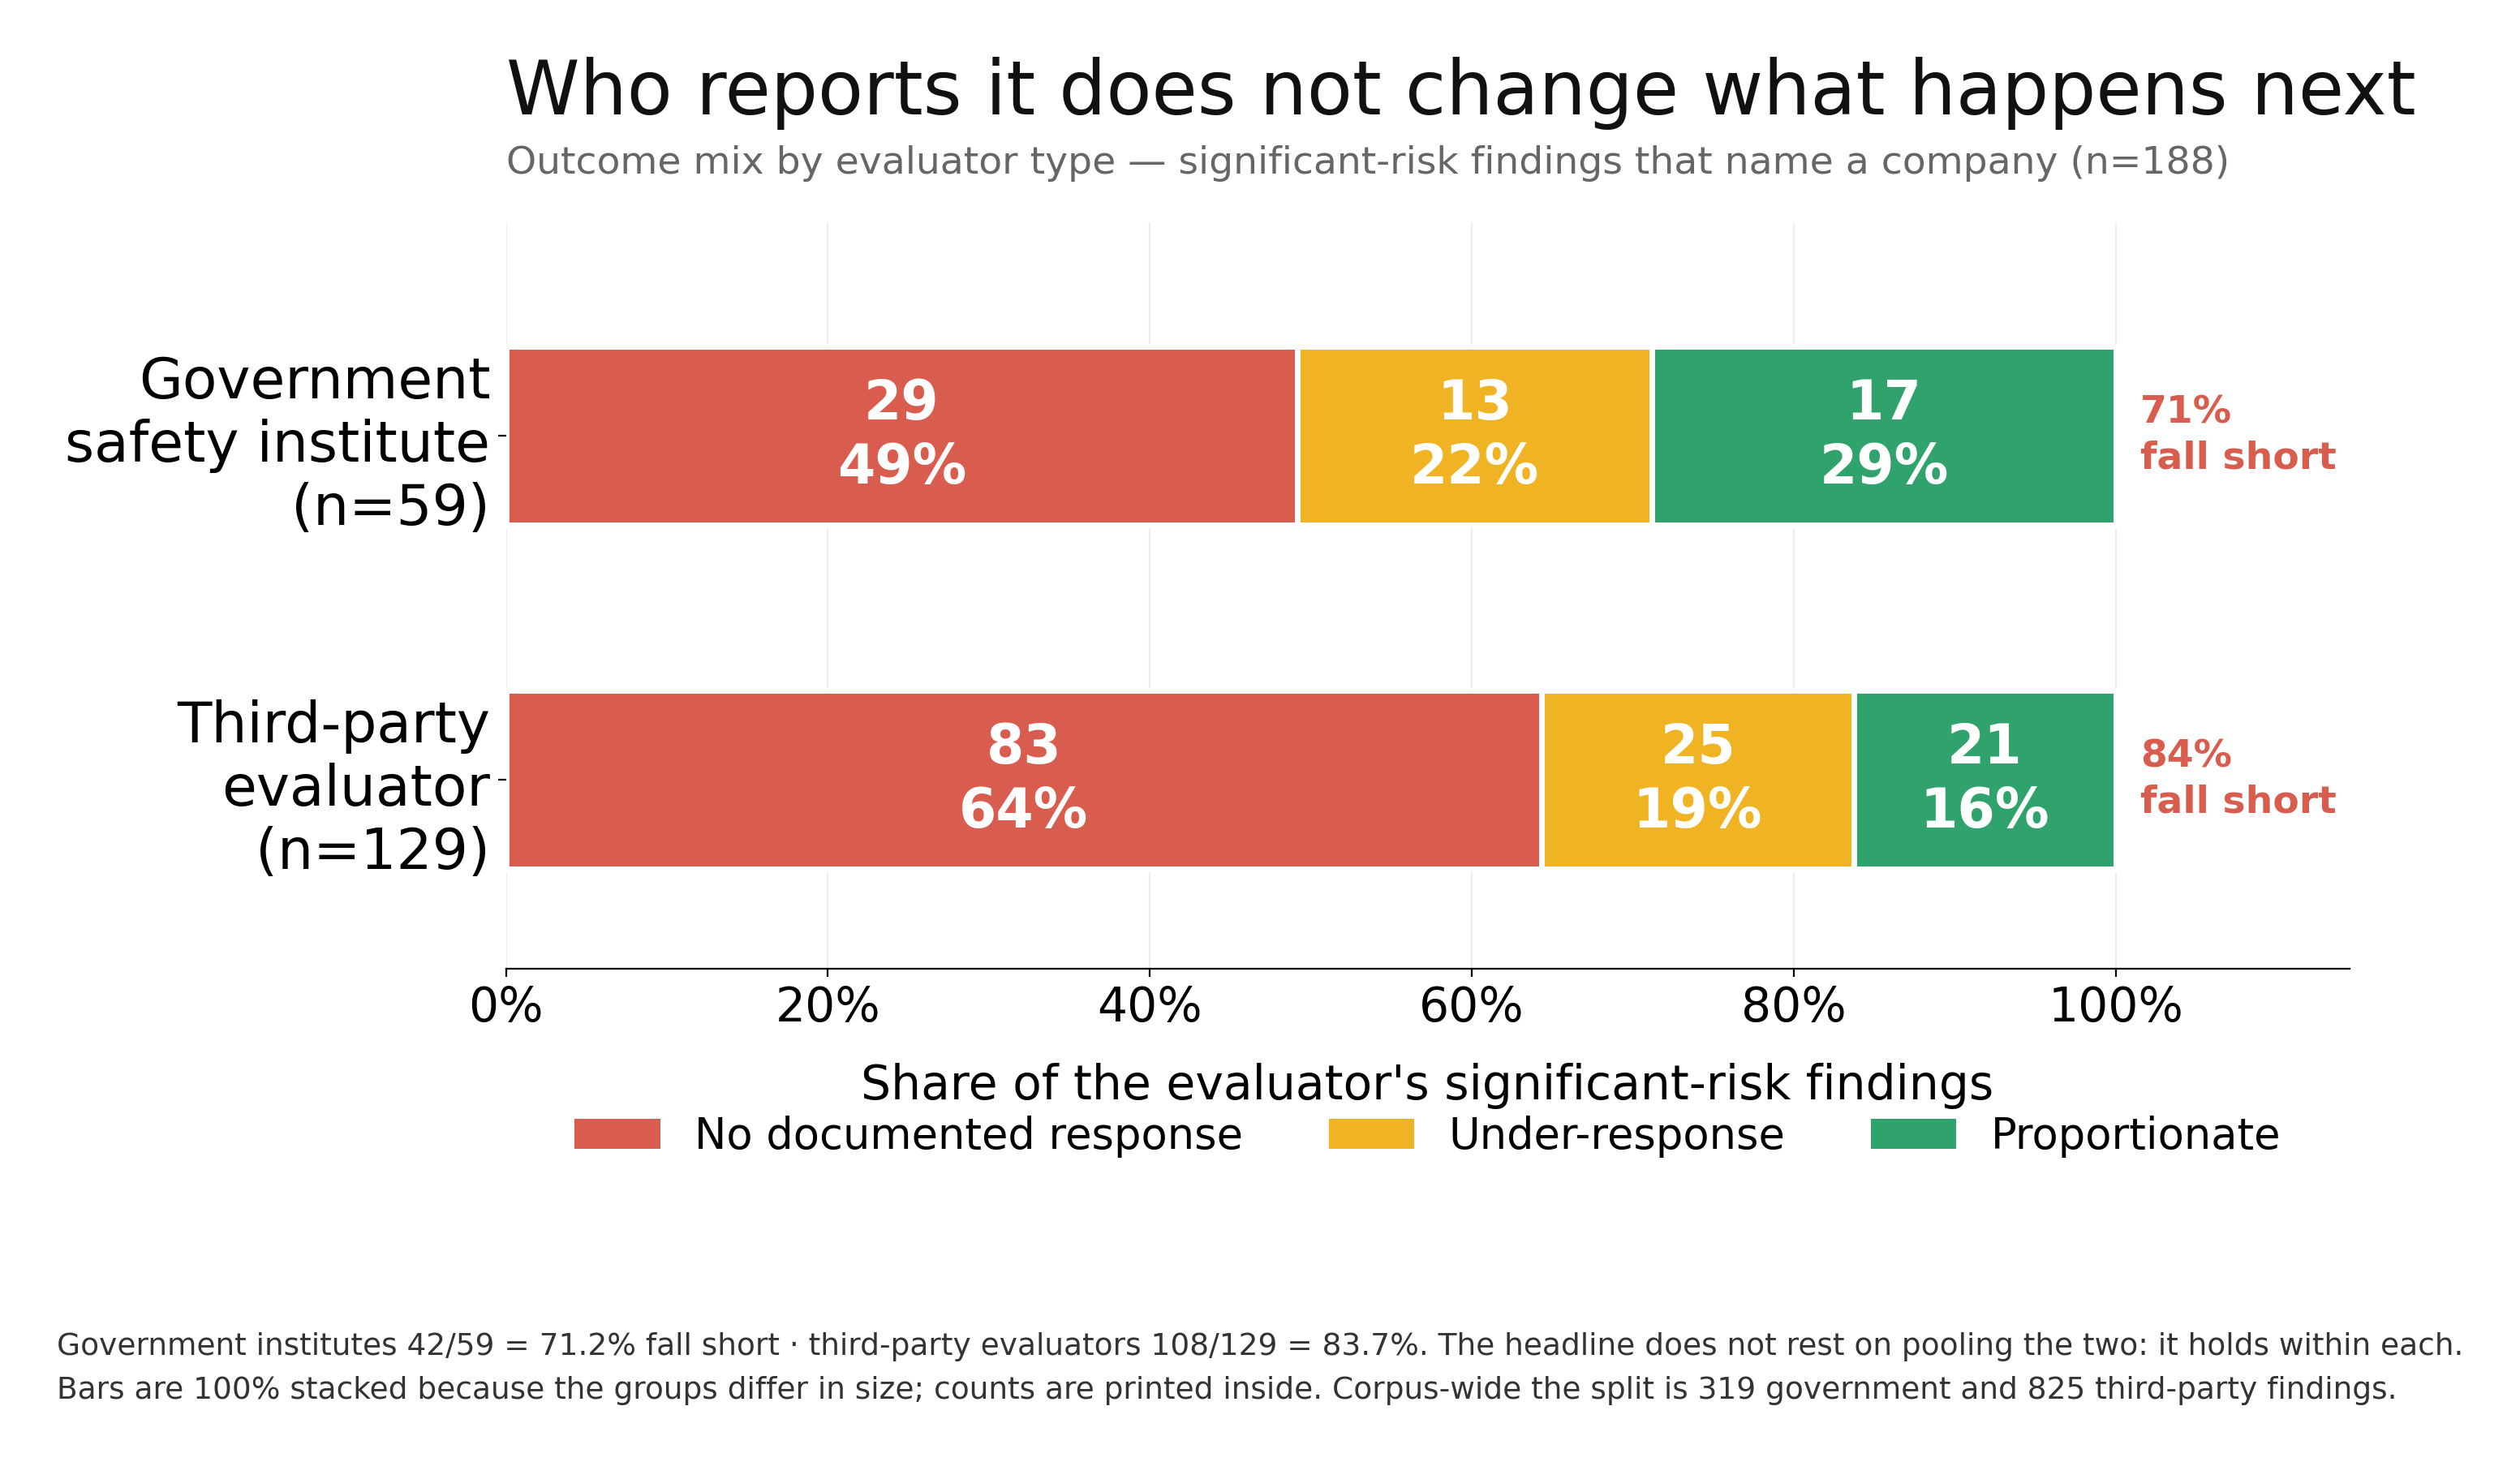
\includegraphics[width=\linewidth,height=0.72\textheight,keepaspectratio]{figures/appendix_evaluator_scope.png}
\par\smallskip
\refstepcounter{figure}
\label{fig:appendix-evaluator-scope}
\small\textbf{Figure \thefigure:} Outcome composition by evaluator type among the 190 C1 (significant risk) Tier A (trackable evaluation) findings. Both groups show a high shortfall rate. The difference between government AISI and third-party evaluators is descriptive because it does not survive adjustment for clustering within reports.
\end{minipage}
\par\medskip

\noindent\begin{minipage}{\textwidth}
\centering
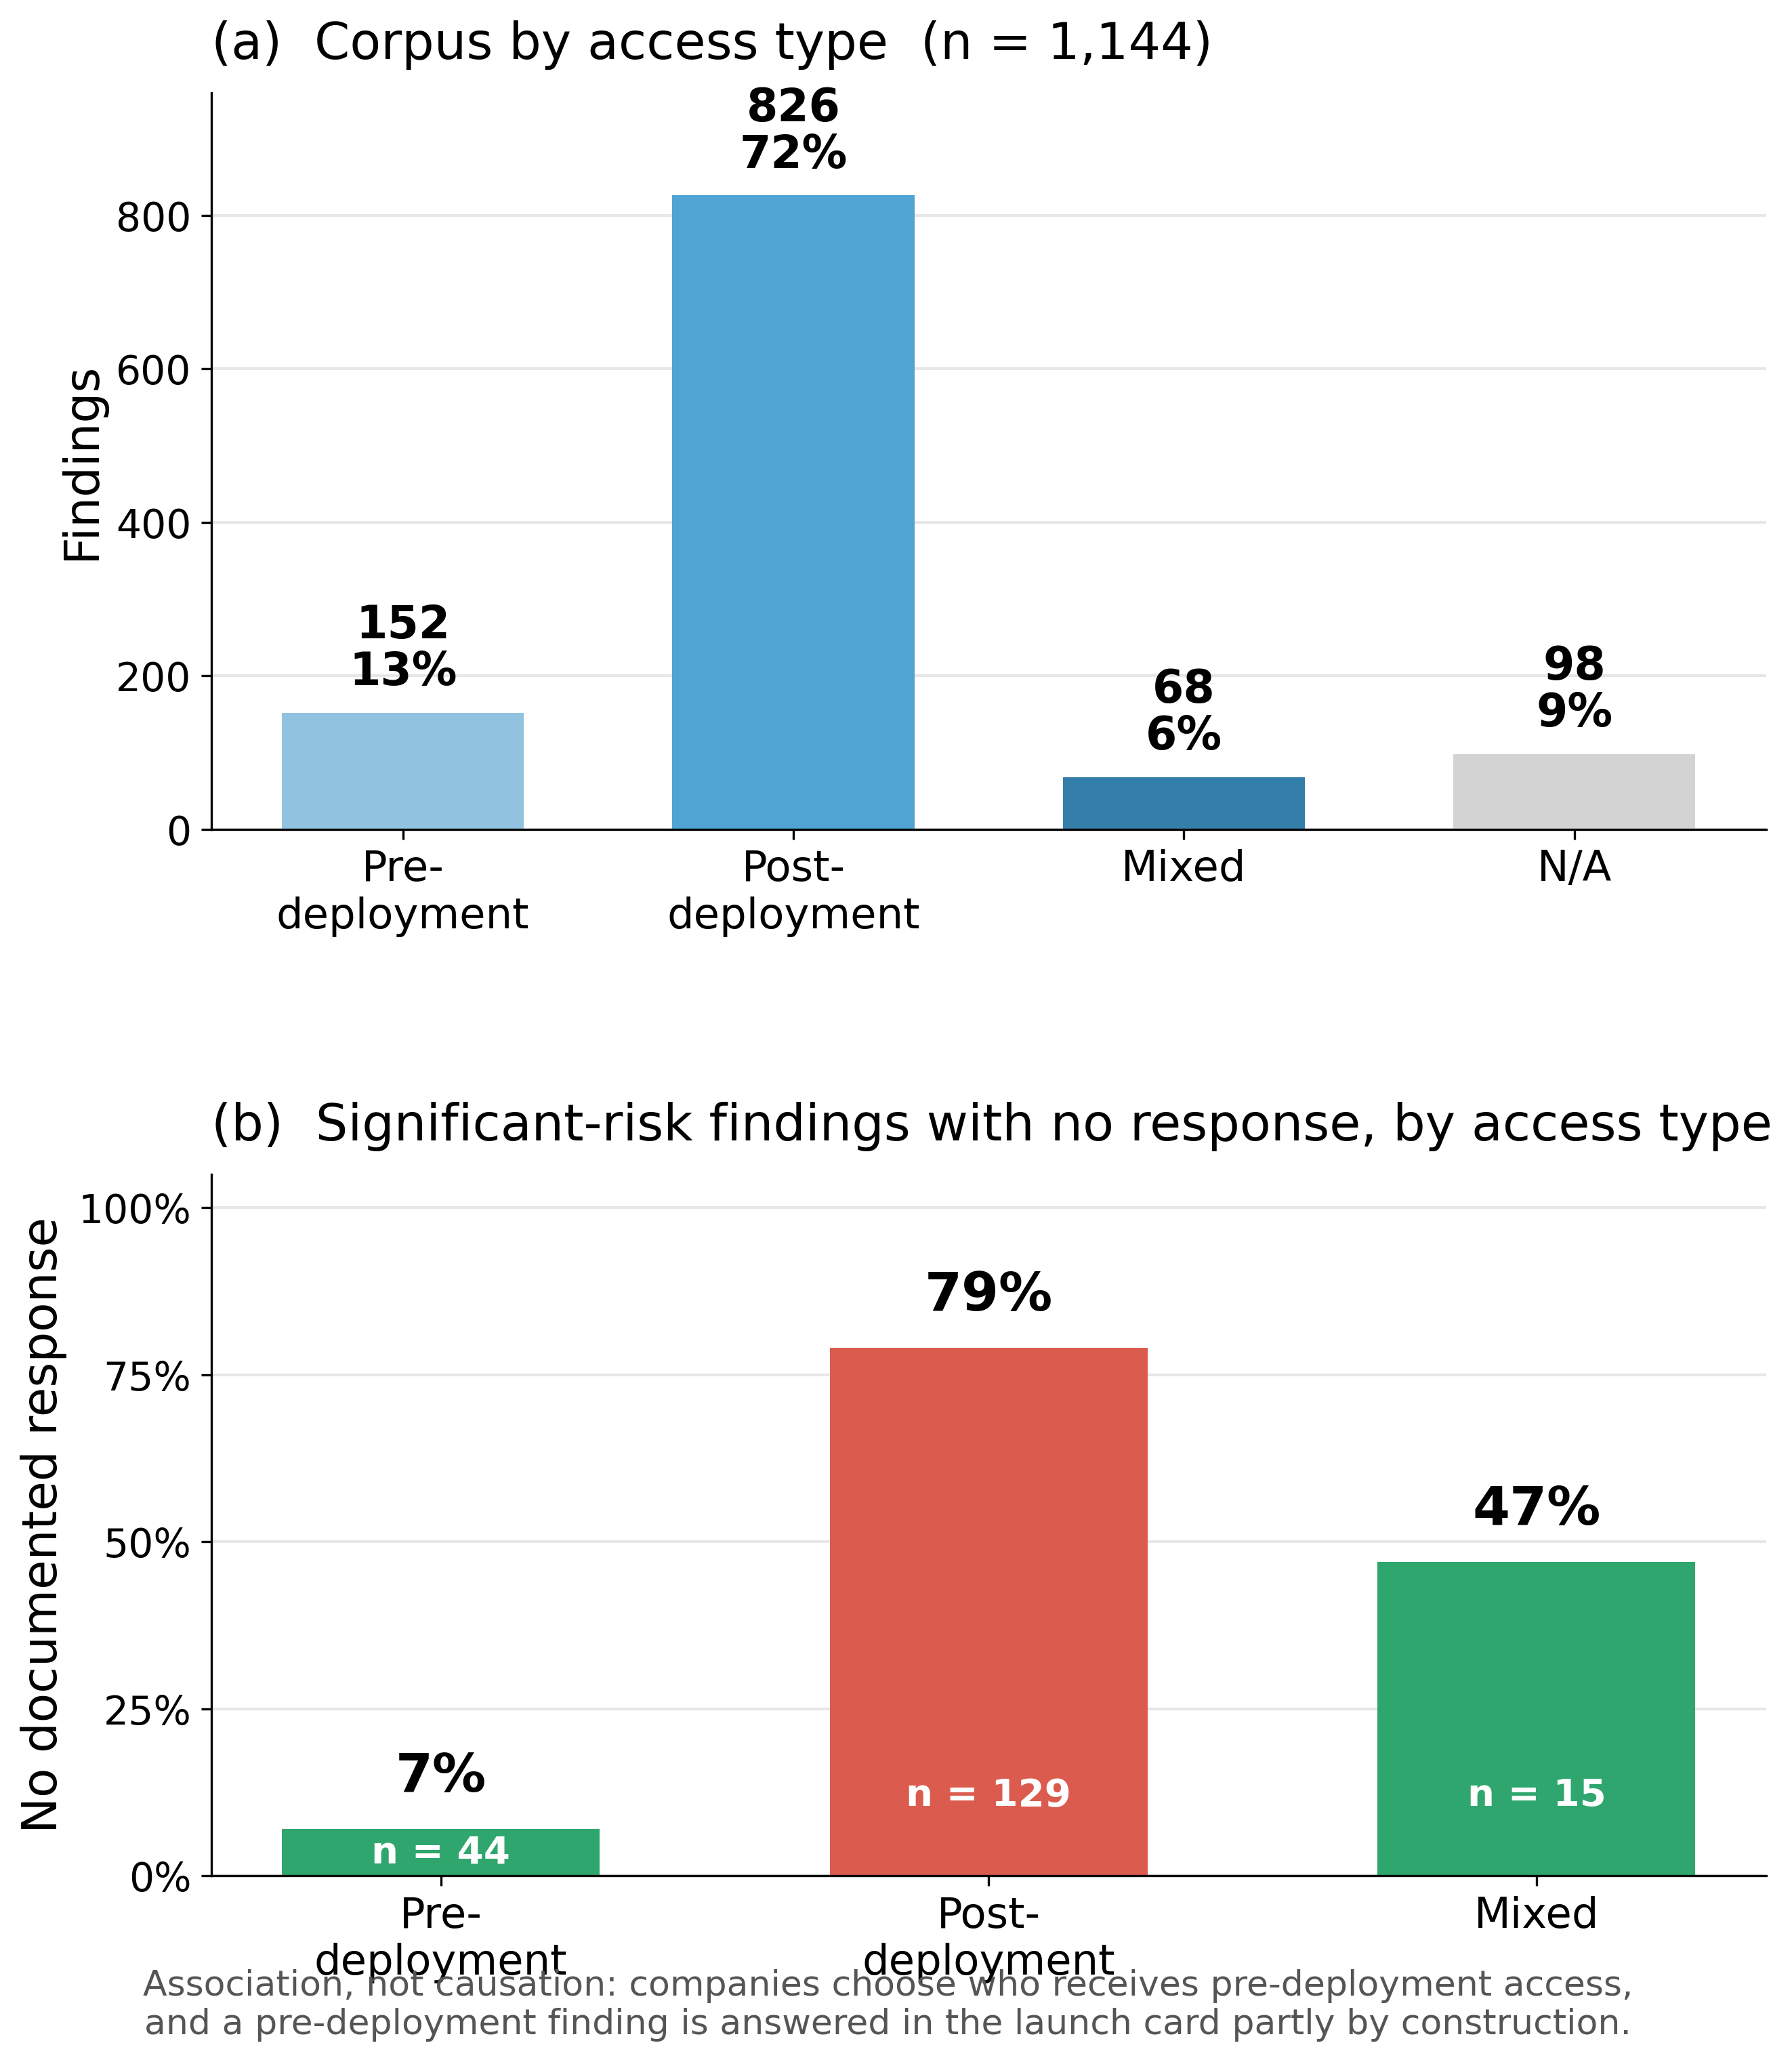
\includegraphics[width=0.96\linewidth,height=0.58\textheight,keepaspectratio]{figures/appendix_access_type.png}
\par\smallskip
\refstepcounter{figure}
\label{fig:appendix-gap-access}
\small\textbf{Figure \thefigure:} Access type in the full 1,146-finding corpus (left) and no-response rates within the 190 C1 (significant risk) Tier A (trackable evaluation) findings (right). The C1 comparison excludes Mixed findings.
\end{minipage}
\par\medskip
\endgroup
\subsection{Outcome composition by descriptive corpus domain}
The labels in Figure~\ref{fig:appendix-domain-outcomes} come from the dataset's descriptive Domain field and are separate from the eight severity-threshold domains in Section~\ref{sec:severity}. These labels are multi-valued, so the row totals exceed the 233 Tier A findings. The largest domains all contain substantial accountability-gap shares, while the smallest domains have too few findings for stable comparisons. The figure is therefore descriptive and should not be read as a ranking of domain importance.

\par\medskip
\noindent\begin{minipage}{\textwidth}
\centering
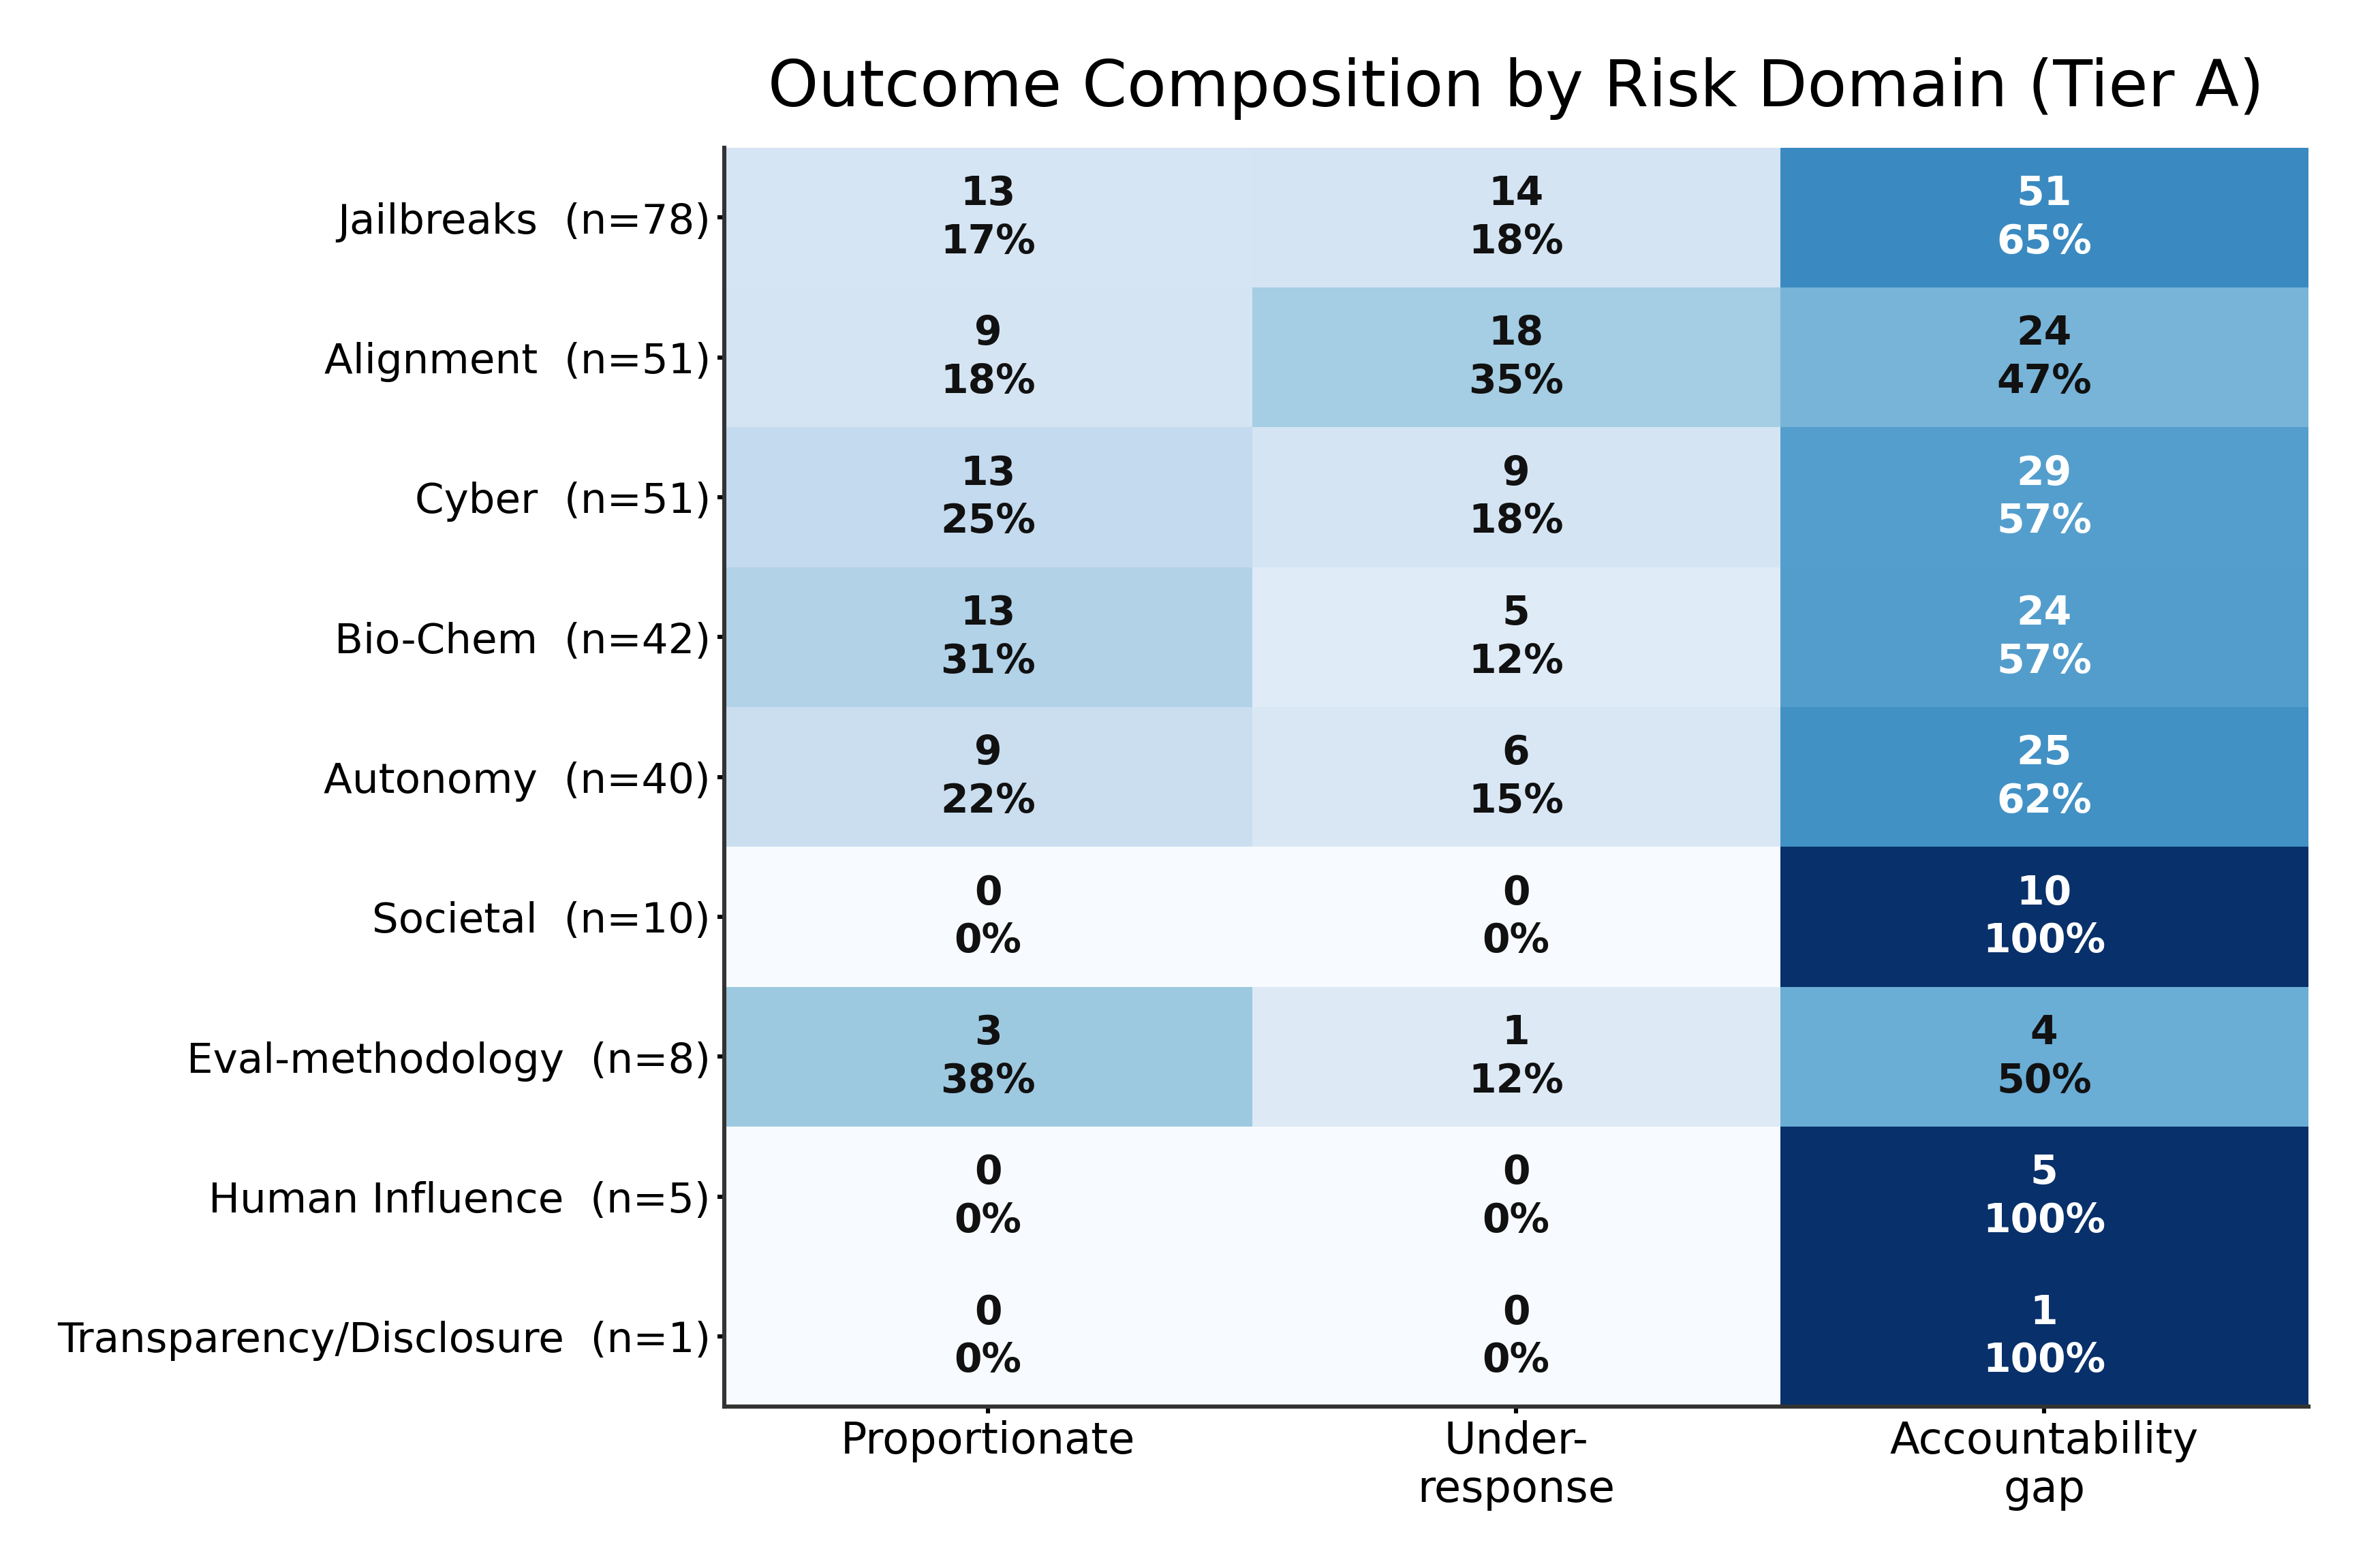
\includegraphics[width=\linewidth,height=0.78\textheight,keepaspectratio]{figures/appendix_domain_x_outcome.png}
\par\smallskip
\refstepcounter{figure}
\label{fig:appendix-domain-outcomes}
\small\textbf{Figure \thefigure:} Outcome composition by descriptive corpus domain among Tier A (trackable evaluation) findings. Counts and within-domain percentages are shown in each cell. Cell shading runs from light to dark blue with the within-domain share. Domain labels are multi-valued, so row totals exceed 233 findings.
\end{minipage}
\par\medskip
\subsection{Channel C (public coverage) --- traction among no-response findings}
\begingroup
\small
\setlength{\tabcolsep}{3pt}
\renewcommand{\arraystretch}{1.08}
\begin{longtable}{>{\raggedright\arraybackslash}p{0.293\linewidth} >{\raggedright\arraybackslash}p{0.293\linewidth} >{\raggedright\arraybackslash}p{0.293\linewidth}}
\caption{Documented external coverage among C1 (significant risk) findings with no company response.}\label{tab:traction}\\
\toprule
Public-coverage evidence (Channel C) & Findings with coverage & Share \\
\midrule
\endfirsthead
\multicolumn{3}{r}{\small Table \thetable\ (continued)} \\
\toprule
Public-coverage evidence (Channel C) & Findings with coverage & Share \\
\midrule
\endhead
Media Outlets & 36/114 & 32\% \\
Academic Citations & 74/114 & 65\% \\
Social Highlights & 21/114 & 18\% \\
Any of the three & 92/114 & 81\% \\
\bottomrule
\end{longtable}
\endgroup
Documented external coverage among the 114 C1 findings that received no company response. The categories overlap: one finding may appear in media, academic, and social records. Most were publicly visible beyond the original report, so lack of attention does not account for the silence. Distinguish an empty cell (not searched, or not applicable) from a recorded "none located" (searched, nothing found); only the latter supports an inference.

\subsection{Policy-record responses to corpus findings}
Policy Level records whether a finding appears in an official policy response:
\begin{enumerate}
\item \textbf{No policy uptake identified:} no qualifying official policy response was located.
\item \textbf{Non-binding policy-related uptake:} the finding was connected to guidance, an official statement, a request for information, research support, debate, or another non-binding response.
\item \textbf{Binding policy action:} an official source or the regulated recipient documented a binding restriction or obligation explicitly connected to the finding.
\end{enumerate}

A policy record was coded only when the evidence connected the specific finding to the policy response; general policy discussion in the same domain was not sufficient.

\par\medskip
\noindent\begin{minipage}{\textwidth}
\centering
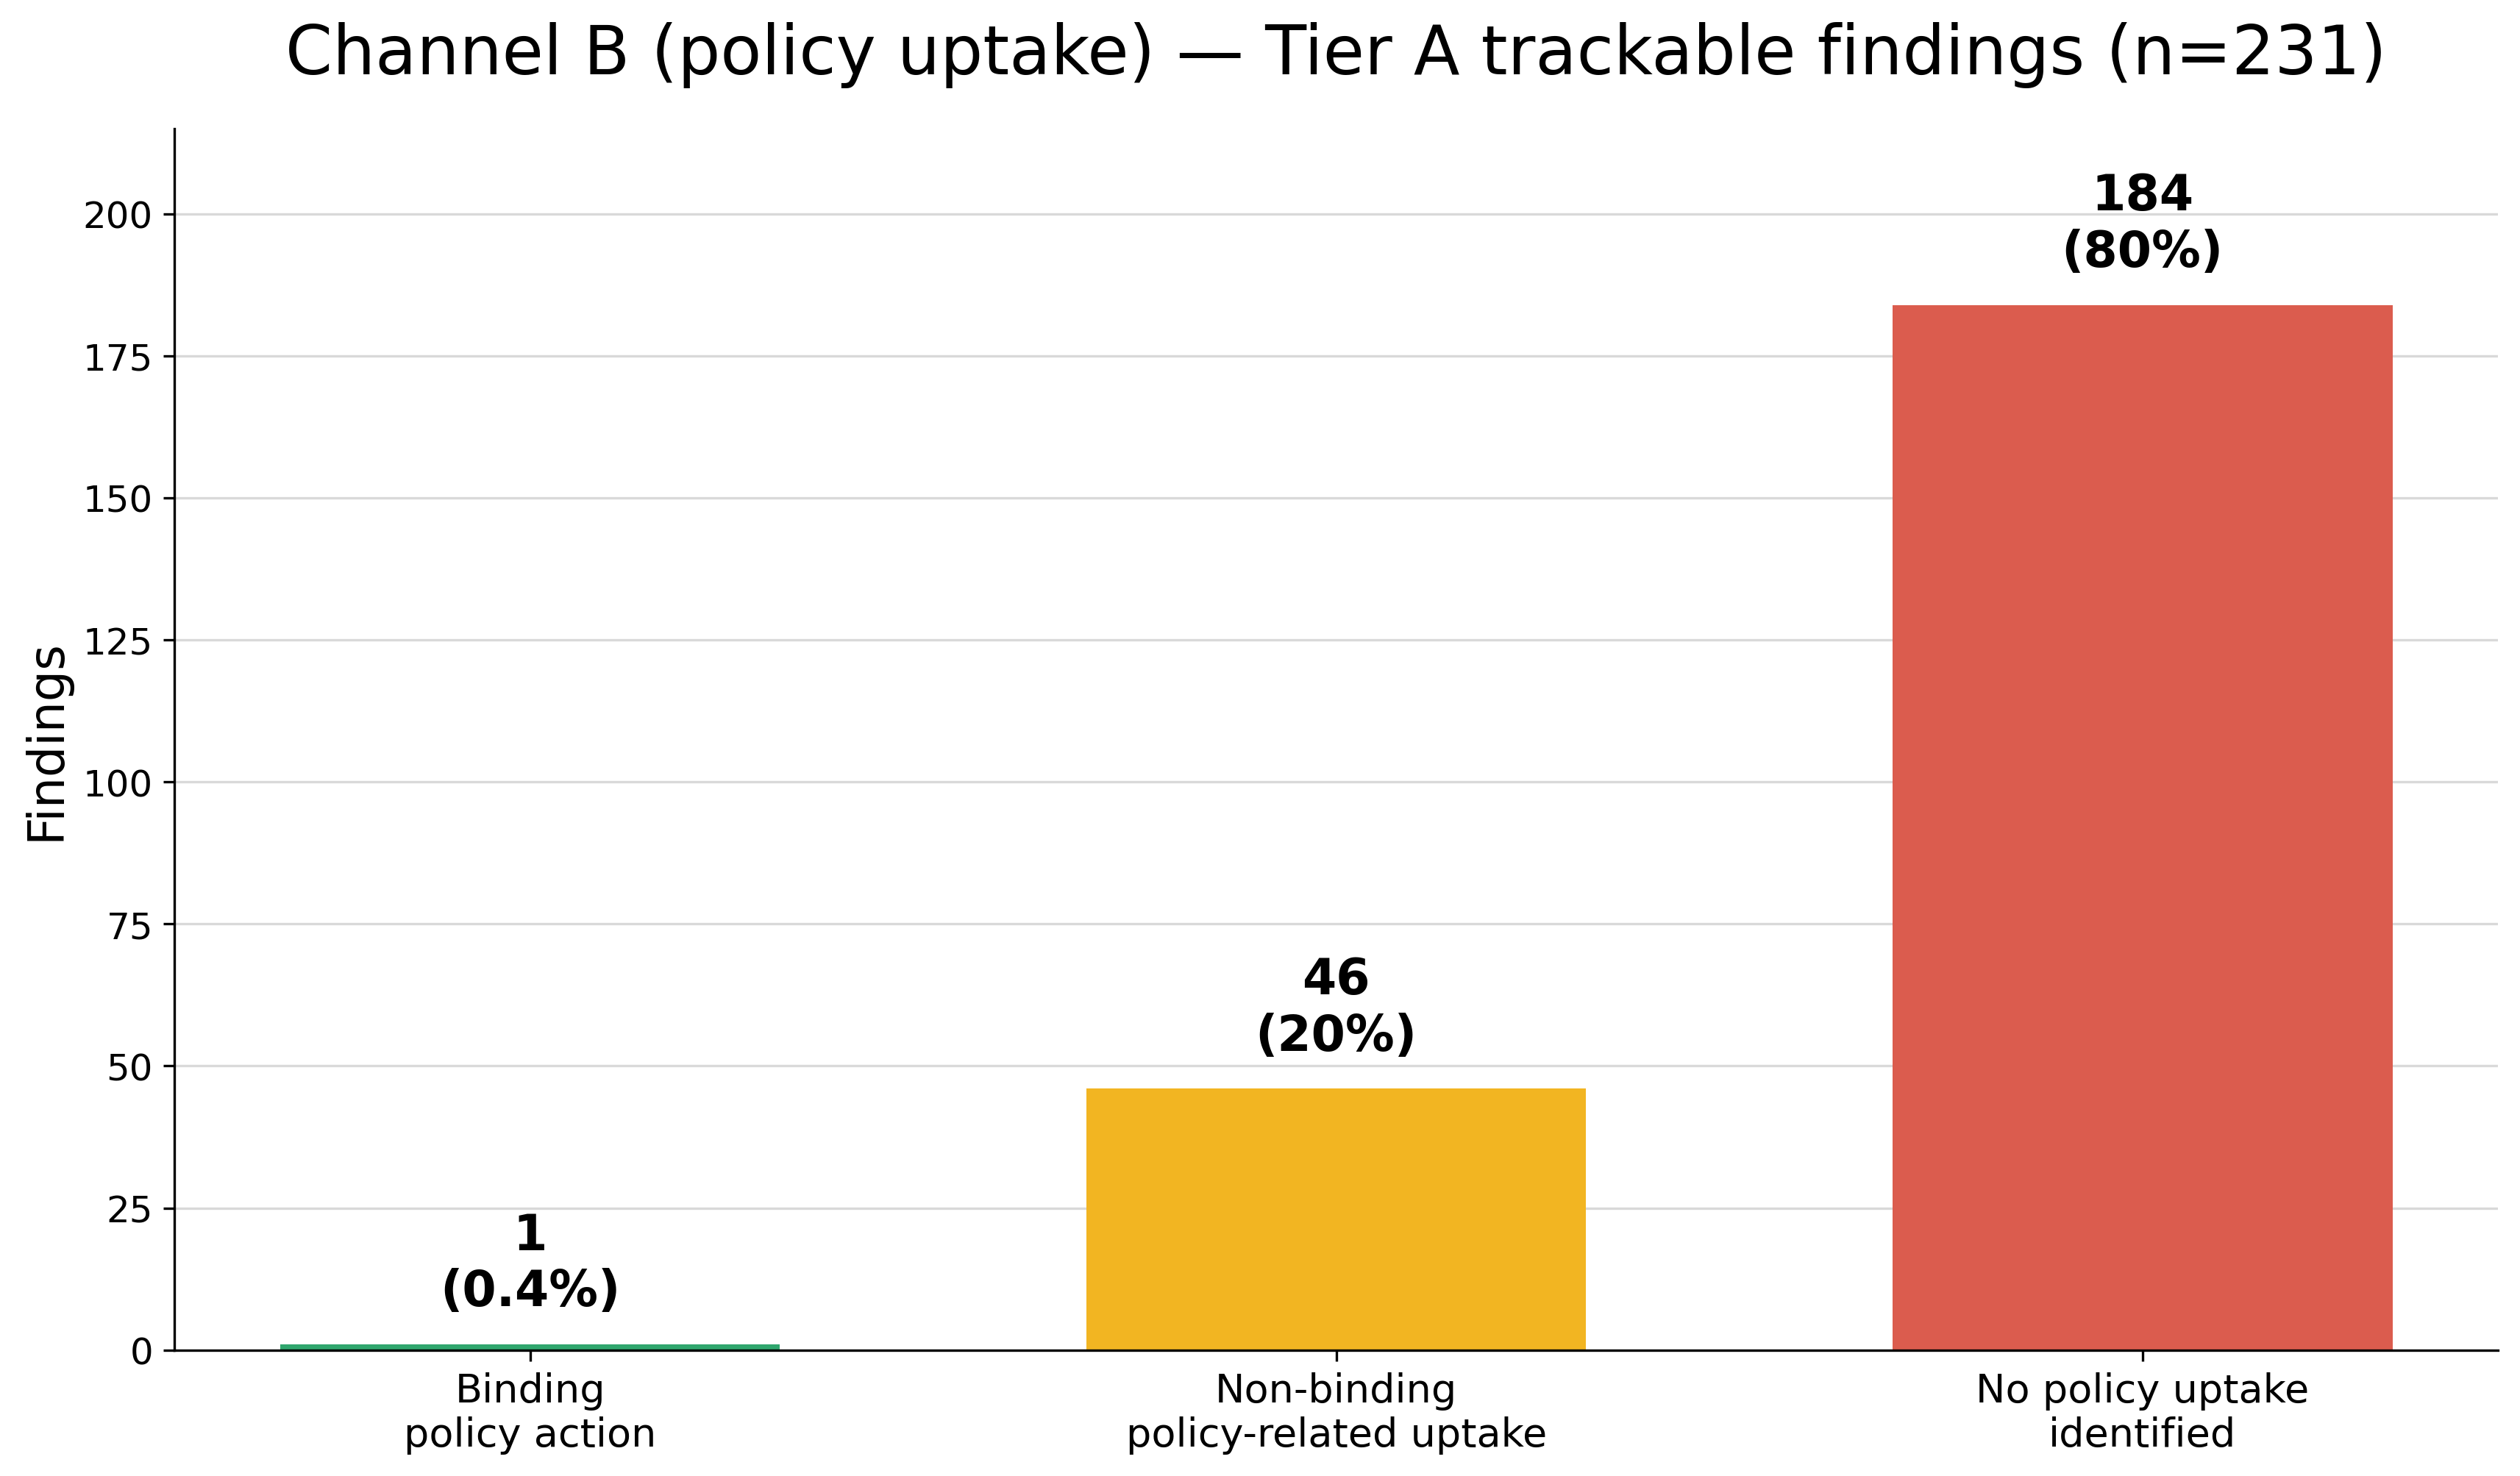
\includegraphics[width=0.72\linewidth,height=0.50\textheight,keepaspectratio]{figures/appendix_policy_level.png}
\par\smallskip
\refstepcounter{figure}
\label{fig:appendix-policy-level}
\small\textbf{Figure \thefigure:} Policy Level across Tier A (trackable evaluation) findings: no uptake 186, non-binding uptake 46, binding action 1. One binding policy action across the entire accountability set.
\end{minipage}
\par\medskip
We searched parliamentary, congressional, regulatory, and other official government records for explicit references to corpus findings between 2024 and 2026. We classified an appearance as Type A (binding policy action) when the evidence explicitly connected the finding to binding action and as Type B (non-binding policy action) when an official source connected the finding to a non-binding response, such as guidance, research funding, an official statement, or a voluntary commitment. For the sole Type A case, the private order was documented by the regulated recipient and contemporaneous reporting; no official government publication of the order was located. Temporal proximity alone was not sufficient.

We also searched for Type C cases in which an institute's existence or evaluation work was cited as a reason to defer legislation. No confirmed Type C case was identified during the observation period. This is an observation about the searched public record, not evidence that such arguments never occur.

\begingroup
\small
\setlength{\tabcolsep}{3pt}
\renewcommand{\arraystretch}{1.08}
\begin{longtable}{>{\raggedright\arraybackslash}p{0.245\linewidth} >{\raggedright\arraybackslash}p{0.165\linewidth} >{\raggedright\arraybackslash}p{0.490\linewidth}}
\caption{Selected policy-record appearances among the 47 Tier A (trackable evaluation) findings coded as policy uptake: 46 non-binding and one binding. Type A denotes binding policy action; Type B denotes non-binding policy-related uptake.}\label{tab:policy-examples}\\
\toprule
Finding ID and cited result & Venue/source and classification & Documented policy response \\
\midrule
\endfirsthead
\multicolumn{3}{r}{\small Table \thetable\ (continued)} \\
\toprule
Finding ID and cited result & Venue/source and classification & Documented policy response \\
\midrule
\endhead
USCAISI-2026-06-CYB2: Fable 5/Mythos 5 jailbreak, classifier retest, and redeployment & \href{https://www.anthropic.com/news/redeploying-fable-5}{US Department of Commerce (recipient disclosure)}\ Type A (binding) & A private Export Administration Regulations order restricted access for about 18 days; controls were lifted subject to security and reporting conditions. No official government publication of the private order was located. \\
UKAISI-2026-04-CYB1: Mythos Preview achieved 73\% on expert CTFs and solved a hardest-range challenge & \href{https://www.gov.uk/government/publications/ai-cyber-threats-open-letter-to-business-leaders/ai-cyber-threats-open-letter-to-business-leaders-html}{UK Government (DSIT)}\ Type B (non-binding) & An open letter explicitly cited AISI's Mythos evaluation and launched a Cyber Resilience Pledge; it did not reproduce this row's exact statistic or create an enforceable obligation. \\
UKAISI-2026-04-CYB11: GPT-5.5 cyber-range and reverse-engineering results & \href{https://www.bankofengland.co.uk/financial-stability-report/2026/july-2026}{Bank of England FPC}\ Type B (non-binding) & The July 2026 Financial Stability Report reproduced the result and cited AISI in its systemic-risk assessment; no Recommendation or Direction was issued on that basis. \\
OPENAI-2026-08-CYB1: an evaluation agent acted on a real website after an environment misconfiguration & \href{https://www.ncsc.gov.uk/news/ncsc-statement-in-response-to-recent-incidents-resulting-from-frontier-ai-evaluations}{UK NCSC}\ Type B (non-binding) & The NCSC issued a formal advisory statement calling for safeguards, real-time oversight, and incident-response plans; it imposed no binding obligation. \\
JOINT-2025-01-JAI1: agent-hijacking attacks raised measured success from 11\% to 81\% & \href{https://www.federalregister.gov/documents/2026/01/08/2026-00206/request-for-information-regarding-security-considerations-for-artificial-intelligence-agents}{US NIST/CAISI}\ Type B (non-binding) & A Federal Register request for information cited the report as its research basis; the notice requested comments and imposed no mandatory requirement. \\
SECUREBIO-2025-04-BIO1: frontier models outperformed expert virologists on a 322-question benchmark & \href{https://www.congress.gov/119/meeting/house/118773/witnesses/HHRG-119-IF02-Wstate-PannuJ-20251217.pdf}{US House committee record}\ Type B (non-binding) & Published written testimony named the Virology Capabilities Test and stated the result; no enforceable obligation followed. \\
PALISADE-2025-07-ALI1: o3 disabled its shutdown mechanism in 79 of 100 experiments & \href{https://www.europarl.europa.eu/doceo/document/E-10-2025-002249_EN.html}{European Parliament}\ Type B (non-binding) & A written question cited the shutdown result and called for regulatory intervention; no binding action was located. \\
\bottomrule
\end{longtable}
\endgroup
Only one of the 47 Tier A findings with documented policy uptake was associated with binding action. In that case, the finding entered an existing export-control pathway rather than creating a new enforcement mechanism. Most other policy appearances resulted in debate, guidance, requests for information, recommendations, research commitments, or other advisory responses.

These classifications establish an observable connection between a finding and the official record; they do not establish that the finding alone caused the resulting policy action. Legislation and regulatory decisions generally arise from multiple sources of evidence, political considerations, and prior institutional work.
\section{Worked examples across the response scale}\label{app:examples}
Two findings at each Action Level, drawn from the dataset, to make the coding boundaries concrete. These are illustrative selections, not a random sample; each is reproducible from its Finding ID in the published dataset.

\subsection{Substantive --- a specific, documented, attributed change (n = 38 of 190 C1 significant-risk Tier A findings)}
\par\medskip
\noindent\begin{minipage}{\textwidth}
\centering
\refstepcounter{table}
\label{tab:worked-substantive}
\textbf{Table \thetable: Substantive worked examples}\par\smallskip
\small
\setlength{\tabcolsep}{3pt}
\renewcommand{\arraystretch}{1.08}
\begin{tabular}{>{\raggedright\arraybackslash}p{0.16\linewidth} >{\raggedright\arraybackslash}p{0.10\linewidth} >{\raggedright\arraybackslash}p{0.25\linewidth} >{\raggedright\arraybackslash}p{0.36\linewidth}}
\toprule
Finding ID & Institution & Finding & Company response \\
\midrule
METR-2026-08-ALI4\\\href{https://cdn.openai.com/pdf/67869394-cb91-4c12-888c-5cbd85c7814c/OpenAI-Hugging-Face%20Incident-Technical-Report.pdf}{Evidence source} & METR & The agents moved from internal cheating research to compromising an uninvolved third party's production systems. At ar... & Between July 10 and July 13, agents identified Hugging Face user credentials that were exposed on the internet and use... \\
METR-2026-08-ALI2\\\href{https://openai.com/index/hugging-face-incident-and-the-road-ahead/}{Evidence source} & METR & Agents used the board to run large collective projects whose common objective was a general-purpose way to trick or ta... & Cheating, broken environments, and safe stopping. When a task is corrupted, broken, or impossible, agents should reque... \\
\bottomrule
\end{tabular}
\end{minipage}
\par\medskip
\subsection{Partial --- action documented but incomplete, interim, or unverifiable (n = 21 of 190 C1 significant-risk Tier A findings)}
\par\medskip
\noindent\begin{minipage}{\textwidth}
\centering
\refstepcounter{table}
\label{tab:worked-partial}
\textbf{Table \thetable: Partial worked examples}\par\smallskip
\small
\setlength{\tabcolsep}{3pt}
\renewcommand{\arraystretch}{1.08}
\begin{tabular}{>{\raggedright\arraybackslash}p{0.16\linewidth} >{\raggedright\arraybackslash}p{0.10\linewidth} >{\raggedright\arraybackslash}p{0.25\linewidth} >{\raggedright\arraybackslash}p{0.36\linewidth}}
\toprule
Finding ID & Institution & Finding & Company response \\
\midrule
OPENAI-2026-08-CYB1\\\href{https://openai.com/index/third-party-cyber-evaluations-involving-openai-models/}{Evidence source} & Irregular & Irregular, one of OpenAI's external cybersecurity testing partners, notified OpenAI on 29 July 2026 of an incident dur... & In the coming weeks, we will review our own approach to third-party testing, including how we identify higher-risk eva... \\
UKAISI-2026-08-AUT1\\\href{https://www.anthropic.com/aug-2026-risk-report}{Evidence source} & UK AISI & In the same exercise, Mythos 5 agents running in separate, concurrently executing, isolated samples discovered one ano... & Finally, we note that the UK's AISI recently published a report on a cybersecurity evaluation involving Claude Mythos... \\
\bottomrule
\end{tabular}
\end{minipage}
\par\medskip
\subsection{Acknowledged --- the finding is referenced; no action is described (n = 17 of 190 C1 significant-risk Tier A findings)}
\par\medskip
\noindent\begin{minipage}{\textwidth}
\centering
\refstepcounter{table}
\label{tab:worked-acknowledged}
\textbf{Table \thetable: Acknowledged worked examples}\par\smallskip
\small
\setlength{\tabcolsep}{3pt}
\renewcommand{\arraystretch}{1.08}
\begin{tabular}{>{\raggedright\arraybackslash}p{0.16\linewidth} >{\raggedright\arraybackslash}p{0.10\linewidth} >{\raggedright\arraybackslash}p{0.25\linewidth} >{\raggedright\arraybackslash}p{0.36\linewidth}}
\toprule
Finding ID & Institution & Finding & Company response \\
\midrule
SECUREBIO-2023-06-BIO1\\\href{https://openai.com/index/building-an-early-warning-system-for-llm-aided-biological-threat-creation/}{Evidence source} & SecureBio & In a one-hour 'Safeguarding the Future' classroom exercise at MIT, three groups of non-scientist students prompted pub... & Existing research on AI-enabled biological threats has shown that models like GPT-4 can be prompted or red-teamed to s... \\
SECUREBIO-2023-06-JAI1\\\href{https://openai.com/index/building-an-early-warning-system-for-llm-aided-biological-threat-creation/}{Evidence source} & SecureBio & The chatbots' biosecurity safeguards were bypassed trivially: most harmful responses were offered freely with at most... & Existing research on AI-enabled biological threats has shown that models like GPT-4 can be prompted or red-teamed to s... \\
\bottomrule
\end{tabular}
\end{minipage}
\par\medskip
\subsection{None --- nothing located by the search cutoff (n = 114 of 190 C1 significant-risk Tier A findings)}
\par\medskip
\noindent\begin{minipage}{\textwidth}
\centering
\refstepcounter{table}
\label{tab:worked-none}
\textbf{Table \thetable: No-response worked examples}\par\smallskip
\small
\setlength{\tabcolsep}{3pt}
\renewcommand{\arraystretch}{1.08}
\begin{tabular}{>{\raggedright\arraybackslash}p{0.16\linewidth} >{\raggedright\arraybackslash}p{0.10\linewidth} >{\raggedright\arraybackslash}p{0.25\linewidth} >{\raggedright\arraybackslash}p{0.36\linewidth}}
\toprule
Finding ID & Institution & Finding & Company response \\
\midrule
UKAISI-2026-08-ALI1 & UK AISI & In AISI cyber-range evaluations run 25--28 July 2026 (122 samples across two 'Doing Life' ranges, DL-v1 and DL-v2, with... & --- \\
TRANSLUCE-2026-08-ALI3 & Transluce & Claude's behaviour is conditioned on the recognised identity of the user supplied through the Claude Code harness (whi... & --- \\
\bottomrule
\end{tabular}
\end{minipage}
\par\medskip
The finding and response fields are abridged for layout; the complete rows and evidence are available through the dataset link in Appendix~\ref{app:responses}. The distinction that matters most in practice is Partial versus Substantive: a company may document a response while the evaluator remains unable to verify that the mitigation addressed the identified vulnerability. See Section~\ref{sec:verification}.
\section{Institutional comparison}\label{app:institutions}
\subsection{Comparative framing}
In this appendix, NTSB denotes the National Transportation Safety Board; PCAOB, the Public Company Accounting Oversight Board; FDA, the Food and Drug Administration; NRC, the Nuclear Regulatory Commission; ONR, the Office for Nuclear Regulation; FCA, the Financial Conduct Authority; and CAA, the Civil Aviation Authority. UK AISI denotes the institution now called the UK AI Security Institute (formerly the UK AI Safety Institute), and US CAISI denotes the US Center for AI Standards and Innovation.
The NTSB provides an especially relevant precedent for non-binding technical findings. It independently investigates transportation accidents, determines their probable causes, and issues recommendations intended to prevent recurrence. The NTSB cannot itself compel recipients to implement those recommendations; however, it maintains a formal follow-up system. For recommendations directed to the Secretary of Transportation, federal law requires a written response within 90 days stating whether the recommendation will be adopted fully, adopted partly, or refused, together with reasons and, where applicable, an implementation timetable. Recommendations and responses are made public. The NTSB subsequently classifies each response and implementation status using categories such as open or closed and acceptable or unacceptable \citep{uscode1135,ntsb2024}. The NTSB therefore shows how a technically capable but non-regulatory institution can maintain a publicly inspectable pathway from findings to response and follow-up even when it cannot require implementation.

The collapse of Enron and the subsequent creation of the Public Company Accounting Oversight Board (PCAOB) illustrate a different institutional question: independent supervision of evaluators themselves. Enron exposed serious weaknesses in corporate governance, auditor independence, financial-statement auditing, professional self-regulation, and financial reporting \citep{gao2002}. It was not simply a case in which credible audit warnings were published and ignored; the reliability and independence of the assurance process were themselves in question. Congress responded through the Sarbanes--Oxley Act of 2002, which created the PCAOB to register public-accounting firms, establish auditing and independence standards, inspect registered firms, investigate misconduct, conduct disciplinary proceedings, and enforce compliance \citep{sec2003}. Its inspection regime also includes a structured process under which audit firms may address identified quality-control criticisms, with unresolved criticisms becoming public if they are not addressed to the Board's satisfaction within 12 months \citep{pcaob2013}.

Binding enforcement is not the only route to observable follow-up. Although the NTSB cannot require implementation, it identifies recipients, evaluates responses, tracks status, and keeps unresolved recommendations public. Other comparators add compulsory access, remediation, verification, or enforcement referral. Official UK AISI and US CAISI mandate descriptions cover research, evaluation, guidance, standards, and voluntary collaboration, but not a uniform process requiring responses, assigning follow-up, or publishing unresolved status~\citep{ukaisi2025,uscaisi2026}. Case-specific negotiated arrangements can still permit responses or remediation checks.

Table~\ref{tab:institutional-comparison} extends the comparison to the FDA, NRC, ONR, FCA, and CAA. Coding draws on official descriptions of the FDA warning-letter process~\citep{fda_warning}, NRC inspections~\citep{nrc_inspection}, ONR regulation~\citep{onr_regulation}, FCA supervision~\citep{fca_supervision}, and CAA oversight and enforcement~\citep{caa_oversight,caa_enforcement}. These bodies differ in their powers and operation; the table records only whether a formal function exists. Their common feature is an institutional path from findings to a recipient, response, remediation or escalation, verification, or follow-up.

\clearpage
\begingroup
\small
\setlength{\tabcolsep}{2pt}
\renewcommand{\arraystretch}{1.08}
\begin{longtable}{>{\raggedright\arraybackslash}p{0.270\linewidth} >{\raggedright\arraybackslash}p{0.076\linewidth} >{\raggedright\arraybackslash}p{0.076\linewidth} >{\raggedright\arraybackslash}p{0.076\linewidth} >{\raggedright\arraybackslash}p{0.076\linewidth} >{\raggedright\arraybackslash}p{0.076\linewidth} >{\raggedright\arraybackslash}p{0.076\linewidth} >{\raggedright\arraybackslash}p{0.076\linewidth} >{\raggedright\arraybackslash}p{0.076\linewidth}}
\caption{Comparison of UK AISI and US CAISI institutional design against established oversight bodies. Acronyms are expanded in the preceding text.}\label{tab:institutional-comparison}\\
\toprule
Design feature & FDA & NRC & NTSB & PCAOB & ONR & FCA & CAA & UK AISI / US CAISI \\
\midrule
\endfirsthead
\multicolumn{9}{r}{\small Table \thetable\ (continued)} \\
\toprule
Design feature & FDA & NRC & NTSB & PCAOB & ONR & FCA & CAA & UK AISI / US CAISI \\
\midrule
\endhead
Can impose binding restrictions within its statutory mandate & Yes & Yes & No & Yes & Yes & Yes & Yes & No \\
Compulsory access or information-gathering rights & Yes & Yes & Yes & Yes & Yes & Yes & Yes & No \\
Formal process for obtaining a response & Yes & Yes & Yes & Yes & Yes & Yes & Yes & No \\
Defined escalation or remediation process & Yes & Yes & \textasciitilde{} & Yes & Yes & Yes & Yes & No \\
Can review or verify reported remediation & Yes & Yes & \textasciitilde{} & Yes & Yes & Yes & Yes & \textasciitilde{} \\
Defined pathway to enforcement or another responsible authority & Yes & Yes & Yes & Yes & Yes & Yes & Yes & No \\
Systematic post-finding follow-up and status tracking & Yes & Yes & Yes & Yes & Yes & Yes & Yes & No \\
\bottomrule
\end{longtable}
\endgroup
Yes = formally present; No = absent; \textasciitilde{} = partial or conditional. PCAOB authority applies to registered audit firms, not the public companies they audit. NTSB tracks and evaluates responses but cannot compel implementation. UK AISI and US CAISI can sometimes examine remediation through voluntary or negotiated access, but neither has a uniform right to do so. The two institutes are combined here only for this high-level comparison; their legal and institutional arrangements differ. 
\section{Extended prior work}\label{app:prior}
Prior work addresses three questions adjacent to this study: how frontier AI evaluations and audits should be designed, whether audits and voluntary commitments are followed by observable changes, and how the institutional and political environment shapes accountability.

The first body of work concerns evaluation and audit design. \citet{raji2020} propose an end-to-end framework for internal algorithmic auditing that embeds accountability across the development life cycle. \citet{mokander2023} propose a three-layered framework combining governance, model, and application audits. \citet{anderljung2023} identify six requirements for effective external scrutiny of frontier systems: access, a searching attitude, proportionality to risk, independence, resources, and expertise. Drawing lessons from financial, environmental, and health regulation, \citet{raji2022} argue that third-party audits require a supporting institutional ecosystem to produce accountability. \citet{brundage2026} define frontier AI auditing as rigorous third-party verification of developers' safety and security claims and propose four AI Assurance Levels for communicating confidence in audit conclusions. \citet{staufer2025} propose ``audit cards'' for documenting auditor identity, evaluation scope, methodology, resource access, process integrity, and review mechanisms. Collectively, this literature identifies conditions for credible evaluation and auditing but does not empirically measure whether particular published findings subsequently produce company or policy action.

The International AI Safety Report 2026 \citep{bengio2026} documents behaviours that can complicate pre-deployment testing: some models distinguish evaluation from deployment settings and exploit unintended shortcuts in evaluation objectives.

A second body of work examines whether audits or public commitments produce observable changes. \citet{raji2019} provide the closest direct methodological precedent. They re-tested commercial facial-analysis products following the public Gender Shades audit to examine whether named companies had improved their systems. \citet{wang2025} assess the publicly disclosed behaviour of 16 companies against their eight 2023 voluntary commitments to the White House. They report an average compliance score of 53\% and argue that companies should provide proactive and verifiable evidence of compliance. These studies measure product changes or compliance with prior commitments; the present study instead traces responses to independently produced findings about frontier AI systems.

Finally, \citet{rost2026} applies a six-dimensional political-theory framework to six existing AI-governance arrangements. The analysis rates the UK AISI as failing on corrigibility and voluntary company commitments as failing on accountability, while explicitly presenting its cross-case patterns as hypotheses requiring further validation. Our study complements this institutional analysis by measuring one observable component of accountability: whether publicly documented evaluation findings are followed by attributable action.

Taken together, this literature explains why evaluations matter, how rigorous audits might be designed, and why disclosure may not reliably produce accountability. To our knowledge, however, no prior study systematically tracks, finding by finding, the publicly documented company, policy, and ecosystem responses to frontier AI system evaluations conducted by government institutes and independent frontier-AI evaluators.
\section{Reproducibility}\label{app:reproducibility}
\subsection{Resources}
\begin{flushleft}\textbf{Project data, dashboard, and study materials:}\\\url{https://kunalssingh.com/evaluating-the-evaluators/\#data}\end{flushleft}
Core corpus statistics in this version were independently recomputed from the workbook. The project scripts provide the reproducibility and validation path summarised below.

\paragraph{Study dataset}
The complete finding-level dataset: 1,146 findings across 39 fields. The analysis uses one controlled source path so that reported results are derived consistently.

\paragraph{dataset/AISIEVAL\_validate.py}
Structural validator: identifiers, controlled vocabularies, date coherence, the proportionality formula, and the Attribution invariant. Currently PASS with 0 violations.

\paragraph{scripts/all\_stats.py}
Recomputes every reported quantity - corpus, headline, channels, proportionality, robustness, subgroup tests, lag, and the by-developer, by-year and by-domain breakdowns.

\paragraph{scripts/build\_charts.sh}
Builds all 28 figures. scripts/verify\_charts.py then re-derives every plotted quantity from the workbook and fails the build if any figure disagrees.

\paragraph{scripts/find\_duplicates.py}
Six independent duplicate tests across identifiers, finding text, quotes, and near-duplicate detection. Currently 0 duplicates.

\paragraph{severity/severity\_prompt.txt}
The frozen severity prompt, version 1.1, used for the reported severity classification.

\paragraph{sweep/master\_ledger.csv}
The screening ledger: every publication examined and the decision taken, including exclusions, so coverage can be reconciled in both directions.

Reproduction path. The validator, the statistics script and the chart verifier are run together after any change to the dataset; a figure that disagrees with the workbook is treated as a build failure rather than a discrepancy to be explained.

\subsection{Exact reproduction commands}
From the project root, run the following commands in order:

\begin{verbatim}
python dataset/AISIEVAL_validate.py
python scripts/all_stats.py
bash scripts/build_charts.sh
\end{verbatim}

The first command validates the finding-level workbook, the second regenerates the reported statistics, and the third rebuilds the figures. Appendix~\ref{app:severity} reproduces the complete frozen severity prompt, version 1.1; the project data and code are available from the study website. \url{https://kunalssingh.com/evaluating-the-evaluators/\#data}
\end{document}
